\documentclass[12pt]{amsart}
\usepackage{amstext,amsfonts,amssymb,amscd,amsbsy,amsmath,verbatim}
\usepackage{ifthen}
\usepackage{color,tikz}

\usepackage{amsthm}
\usepackage{latexsym}
\usepackage[all]{xy}
\usepackage{enumerate}
\usepackage{url}
\usepackage{subcaption}
\usepackage{float}


\newtheorem{lemma}{Lemma}[section]
\newtheorem{theorem}[lemma]{Theorem}
\newtheorem{propo}[lemma]{Proposition}

\newtheorem{prop}[lemma]{Proposition}
\newtheorem{cor}[lemma]{Corollary}
\newtheorem{conj}[lemma]{Conjecture}
\newtheorem{claim}[lemma]{Claim}
\newtheorem{claim*}{Claim}
\newtheorem{thm}[lemma]{Theorem}
\newtheorem{defn}[lemma]{Definition}
\newtheorem{example}[lemma]{Example}
\newtheorem{definition}[lemma]{Definition}
\newtheorem{problem}[lemma]{Problem}
\newtheorem*{problem*}{Problem}


\theoremstyle{remark}
\newtheorem{remark}[lemma]{Remark}

\usepackage{geometry,enumerate}
\geometry{a4paper, top=3.5cm, bottom=3cm, left=3cm, right=3cm}

\parindent = 6pt
\parskip = 4pt

% Commands
\newcommand{\isom}{\cong}
\newcommand{\m}{\mathfrak m}
\newcommand{\lideal}{\langle}
\newcommand{\rideal}{\rangle}
\newcommand{\initial}{\operatorname{in}}
\newcommand{\Hilb}{\operatorname{Hilb}}
\newcommand{\Spec}{\operatorname{Spec}}
\newcommand{\im}{\operatorname{im}}
\newcommand{\NS}{\operatorname{NS}}
\newcommand{\Frac}{\operatorname{Frac}}
\newcommand{\ch}{\operatorname{char}}
\newcommand{\Proj}{\operatorname{Proj}}
\newcommand{\id}{\operatorname{id}}
\newcommand{\Div}{\operatorname{Div}}
\newcommand{\tr}{\operatorname{tr}}
\newcommand{\Tr}{\operatorname{Tr}}
\newcommand{\Supp}{\operatorname{Supp}}
\newcommand{\Gal}{\operatorname{Gal}}
\newcommand{\Pic}{\operatorname{Pic}}
\newcommand{\QQbar}{{\overline{\mathbb Q}}}
\newcommand{\Br}{\operatorname{Br}}
\newcommand{\Bl}{\operatorname{Bl}}
\newcommand{\cF}{\mathcal{F}}
\newcommand{\NN}{\mathbb{N}}
\newcommand{\grad}{\nabla}
\DeclareMathOperator*{\argmin}{arg\,min}

\newcommand{\Cox}{\operatorname{Cox}}
\newcommand{\Tor}{\operatorname{Tor}}
\newcommand{\diam}{\operatorname{diam}}
\newcommand{\Hom}{\operatorname{Hom}} %done
\newcommand{\sheafHom}{\mathcal{H}om}
\newcommand{\Gr}{\operatorname{Gr}}
\newcommand{\Osh}{{\mathcal O}}
\newcommand{\kk}{\kappa}
\newcommand{\rank}{\operatorname{rank}}
\newcommand{\prox}{\operatorname{prox}}

\newcommand{\codim}{\operatorname{codim}}
\newcommand{\conv}{\operatorname{conv}}
\newcommand{\D}{{\mathcal D}}
\newcommand{\PP}{\mathbb{P}}
\newcommand{\EE}{\mathbb{E}}

\newcommand{\RR}{\mathbb{R}}
\newcommand{\zz}{\mathbb{Z}}
\newcommand{\Sym}{\operatorname{Sym}} %done
\newcommand{\GL}{{GL}}
\newcommand{\grG}{{\mathcal{G}}}

\newcommand{\Syz}{\operatorname{Syz}}
\newcommand{\defi}[1]{\textsf{#1}} % for defined terms


\newcommand{\Bmod}{\ensuremath{B_
\text{mod}}}
\newcommand{\Bint}{\ensuremath{B_\text{int}}}
\newcommand\commentr[1]{{\color{red} \sf [#1]}}
\newcommand\commentb[1]{{\color{blue} \sf [#1]}}
\newcommand\commentm[1]{{\color{magenta} \sf [#1]}}
\newcommand{\ddr}[1]{{\color{blue} \sf $\clubsuit\clubsuit\clubsuit$ Daniel: [#1]}} 
\newcommand{\mv}[1]{{\color{red} \sf $\clubsuit\clubsuit\clubsuit$ Mauricio: [#1]}}

\begin{document}

\author{Daniel De Roux}
\address{
Departamento de matem\'aticas\\
Universidad de los Andes\\
Carrera $1^{\rm ra}\#18A-12$\\ 
Bogot\'a, Colombia
}
\email{d.de1033@uniandes.edu.co}

\author{Mauricio Velasco}
\address{
Departamento de matem\'aticas\\
Universidad de los Andes\\
Carrera $1^{\rm ra}\#18A-12$\\ 
Bogot\'a, Colombia
}
\email{mvelasco@uniandes.edu.co}

\subjclass[2000]{Primary 15A29 % Inverse problems
Secondary 15B52,52A22} % Random matrices, Random Convex sets and integral geometry
\keywords{Compressed sensing, truncated moment problems, Kostlan-Shub-Smale polynomials}

\begin{abstract} We study the problem of learning the cluster structure of a random graph $\grG$ from an independent sample. We propose a Wasserstein robust formulation of this optimization problem and prove that it leads to a tractable convex optimization problem. We give theoretical exact recovery guarantees for this problem when the Wasserstein metric is induced by the nuclear norm and $\grG$ is distributed according to the stochastic block model. Finally we present our Julia implementation of the proposed algorithm and show its numerical performance on synthetic data.
\end{abstract} 

\title{Graph clustering and the nuclear Wasserstein metric.}
\maketitle

\section{Introduction}


Let $\grG$ be a random graph with $n$ vertices. By a deterministic summary of $\grG$ we mean a (deterministic) graph $H^*$ which, on average, differs from $\grG$ by as few edges as possible. In this article we study the problem of finding deterministic summaries {\it from an independent sample} of $\grG$ of size $N$. More precisely we address the following problem:

\begin{problem}\label{Prob} Given adjacency matrices $B_1,\dots, B_N$ of an independent sample of $\grG$ find a symmetric matrix $A^*$ in $\argmin_A \EE_{B\sim \grG}[\|A-B\|_1]$. 
\end{problem}

Special cases of this problem arise in cluster detection and in data summarization, both heavily studied in the literature (see Section~\ref{Sec: PreviousWork} for details).

A possible approach to problem~\ref{Prob} is to use the samples to construct the empirical measure $\hat{\mu}:=\sum_{i=1}^N \frac{1}{N}\delta_{B_i}$ as an approximation of the distribution of $\grG$ and to find a minimizer $A$ of the resulting empirical risk
\[ \EE_{B\sim \mu}[\|A-B\|_1]=\frac{1}{N}\sum_{i=1}^N \|A-B_i\|_1.\]

This approach is consistent and will lead to an optimal solution as the sample size $N\rightarrow \infty$. However, when the sample size $N$ is not sufficienly large (typicaly one has few samples of very large graphs) for $\hat{\mu}$ to be a good approximation for the distribution of $\grG$ this approach leads to overfitting. To mitigate this problem we propose a robust version of Problem~\ref{Prob}. In the robust version one aims to minimize the worst-case risk when the distribution of $B$ is allowed to vary in a ball $\mathcal{N}_{\delta}(\hat{\mu})$ of radius $\delta>0$ centered at the empirical measure $\hat{\mu}$ in a suitable metric, leading to 

\begin{problem}\label{ProbRobusto} Given adjacency matrices $B_1,\dots, B_N$ of an independent sample of $\grG$ find a symmetric matrix $\overline{A}$ which minimizes the robust worst-case risk 
\[R_{\delta}(A):=\left(\sup_{\nu\in \mathcal{N}_{\delta}(\hat{\mu})} \EE_{B\sim \grG}[\|A-B\|_1]\right).\] 
\end{problem}
The robust worst-case risk is obviously dependent on the chosen metric among probability distributions. In this article we will use the Wasserstein metric $W_{\|\bullet\|}$ induced by a norm $\|\bullet\|$ on the space $K$ of symmetric matrices with entries in $[0,1]$. More precisely, if $\nu_1,\nu_2$ are probability measures on $K$ and $\Pi(\nu_1,\nu_2)$ is the set of random variables $(Z_1,Z_2)$ taking values in $K\times K$  with $Z_i\sim \nu_i$ then the Wasserstein distance between $\nu_1$ and $\nu_2$ is given by 
\[ W_{\|\bullet\|}(\nu_1,\nu_2):=\inf_{(Z_1,Z_2)\in \Pi(\nu_1,\nu_2)} \EE[\|Z_1-Z_2\|].\]

The seminal work of Esfahani and Kuhn~\cite{EsfahaniKuhn} shows that robust formulations defined using the Wasserstein metric often lead to tractable convex optimization problems. Our first result is that this is also true for Problem~\ref{ProbRobusto} when the Wasserstein metric is induced by any semidefinitely representable norm.

\begin{theorem}\label{thm: finiteConvex} Let $K$ be the set of $n\times n$ symmetric matrices with entries in $[0,1]$, let $\|\bullet\|$ be a norm on $K$ and let $\delta>0$. Problem~\ref{ProbRobusto} is equivalent to:
\[\min_{(A,s_1,\dots, s_N,\lambda)\in \mathcal{T}}\left( \lambda\delta +\frac{1}{N}\sum_{i=1}^N s_i \right)\]
where $\mathcal{T}$ is the set of $(A,\vec{s},\lambda)\in K\times \RR^n\times \RR$  satisfying the inequalities $\lambda\geq 0$ and $\eta_{E, i}(\lambda)\leq s_i$ as $i=1,\dots, N$ and $E$ ranges over the set of all $\{-1,1\}$-symmetric matrices, where
\[\eta_{E, i}(\lambda):= \sup_{Y\in K} \left(\langle E, A-Y\rangle -\lambda \|B_i-Y\|\right)\]
\end{theorem}

The reformulation in Theorem~\ref{thm: finiteConvex} transforms the problem into a finite-dimensional convex optimization problem which unfortunately contains  an exponential number of constraints. To address this problem we introduce:
\begin{enumerate}
\item A more tractable simplification which agrees with the original problem whenever the optimal $\overline{A}$ occurs at a matrix with entries in $\{0,1\}$.
\item A relaxation of $(1)$ which takes the form of a regularized empirical risk minimization problem.
\end{enumerate}
leading to practical algorithms for graph summarization. More specifically, if $\mathcal{S}^{n\times n}$ denotes the space of real symmetric $n\times n$ matrices we prove the following 

\begin{theorem}\label{Thm: tractable}If $A$ is a symmetric $\{0,1\}$-matrix and $\delta>0$ then:
\begin{enumerate}
\item{  The following equality holds:
\[
R_{\delta}(A)=\min_{\mathcal{H}} \left(\lambda\delta +\frac{1}{N}\sum_{i=1}^N s_i+\frac{1}{N}\sum_{i=1}^N\|A-B_i\|_1\right)
\]
where $\mathcal{H}$ is the set of $(\lambda, s_1,\dots, s_N,\Lambda, W)\in \RR\times\RR^N\times \mathcal{S}^{n\times n} \times \mathcal{S}^{n\times n}$ which satisfy the inequalities:
\[
\begin{array}{l}
\|W\|_{*}\leq \lambda\\
\Lambda \geq 0\\
2A-11^t-W + \Lambda \geq 0\\
\|\Lambda\|_{1}\leq s_i-\langle 2A-11^t-W, B_i\rangle\text{ for $i=1,\dots, N$}
\end{array}
\]}
\item The following inequality holds:
\[R_{\delta}(A)\leq \frac{1}{N}\sum_{i=1}^N\|A-B_i\|_1+ \delta\|2A-11^t\|_*.\]
\end{enumerate}
Moreover, if $\|\cdot\|$ is a semidefinitely representable function then both $(1)$ and the minimization of the right hand side of $(2)$ for $A\in K$ are semidefinite programming problems.
\end{theorem}

Solving the optimization problems in Theorem~\ref{Thm: tractable} leads to a new algorithm for estimating deterministic graph summaries which we call {\it Wasserstein robust graph summarization}. We carried out extensive numerical experiments applying this algorithm to a variety of graphs $G$ distributed according to the stochastic block model and observed that the regularized problem with the Wasserstein metric {\it induced by the spectral norm} was able to recover the correct cluster structure using only very few samples outperforming all others. This leads us to propose the {\it Wasserstein robust nuclear norm summarization problem}, given by

\begin{equation}\label{WRNNS}
\min_{A\in K} \left(\frac{1}{N}\sum_{i=1}^N\|A-B_i\|_1+ \delta\|2A-11^t\|_*\right) 
\end{equation}

where the nuclear norm $\|B\|_*$ of a matrix $B$ is the dual of the spectral norm and equals the sum of its singular values.

A central result of this article is an exact recovery guarantee for this algorithm. 
More precisely, we show that exact recovery occurs for suitable $\delta>0$ with overwhelming probability on samples distributed according to the stochastic block model, explaining the good practical performance of Wasserstein nuclear norm summarization in cluster detection. In order to describe our exactness guarantee we need to establish notation for the parameters of the stochastic block model. Recall that a random graph $\grG$ has distribution given by the stochastic block model in $n$ vertices if there is a partition of $[n]$ into disjoint subsets $C_1,\dots, C_k$, real numbers $0\leq q<\frac{1}{2}<p_1,\dots, p_k\leq 1$ and edges are added independently with probability $p_{ij}$ of joining vertices $i,j$ given by
\[p_{ij}:=\begin{cases}
p_t\text{, if $\{i,j\}\subseteq C_t$}\\
q\text{, else.}
\end{cases}
\] 
Such a random graph $\grG$ has a unique deterministic summary $A^*$ obtained by putting edges only between vertices belonging to the same cluster.

\begin{theorem}\label{thm. performance} Assume $\grG$ is a stochastic block model with $\ell=2$ clusters. Suppose $B_1,\dots, B_N$ are independent and are distributed according to $\grG$. If $\alpha = \min (|p_t-\frac{1}{2}|, |q-\frac{1}{2}|)$, $\delta^*=\frac{n\alpha}{4}$ and $a(\delta):=\frac{\delta\left(\alpha-\frac{\delta}{n}\right)^2}{n\left(1+\frac{2\delta}{n}\right)}$ then the probability that $A^*$ is not the unique minimizer of~(\ref{WRNNS}) is bounded above by
\[ \exp\left(-\frac{2N(n-1)^3(\alpha n-\delta^*)^2}{n}\right) + e^{-N\left(\delta^* a(\delta^*)\right)}\prod_{i\neq j}\left(1+ (e^{-4a}\widetilde{p_{ij}}+\widetilde{q_{ij}})^{\frac{N}{2}}\right).\] 
which decreases exponentially with the sample size $N$.
\end{theorem}

The key point of the proof of Theorem~\ref{thm. performance}, discussed at length in Section~\ref{Clustering}, is that the subdifferential of the regularization term at $A^*$ is sufficiently rich so as to contain enough transportation matrices. This gives a geometric explanation for why the nuclear norm is a good regularizer for graph summarization problems.
 
Finally we focus on the practical performance of the proposed algorithm. Solving the optimization problems appearing in Theorem~\ref{Thm: tractable} typically require solving large semidefinite programs which are beyond the  capacity of standard off-the-shelf software even for relatively small graphs (of say $40$ vertices with $N=4$). One possible reason is that off-the-shelf solvers often use interior point methods, which are highly accurate but often do not scale well. A better alternative, especially well suited for Wasserstein robust nuclear norm summarization is to use first order numerical optimization methods such as the alternating direction method of multipliers (ADMM). In Section~\ref{Numerics} we adapt the ADMM algorithm to our regularized problem and present our open source Julia implementation. This implementation can run the Wasserstein nuclear norm summarization algorithm in graphs of up to 10000 vertices and $N\leq 10$ on a common laptop. 

\subsection{Relation to previous work.}
\label{Sec: PreviousWork}

Understanding structural properties of graphs is a problem of high interest since these appear naturally in many areas. The problem of finding communities in a graph is one of the most studied tasks in machine learning, with  applications to Biology \cite{cabreros2016detecting, cline2007integration,xu2002clustering}, social data understanding \cite{domingos2001mining,mishra2007clustering,newman2002random} and other general machine learning tasks such as natural language processing \cite{collobert2011natural,ratinov2009design}. Most theoretical results in the community detection problem occur in the context of generative random graph models. Of these the most studied is the stochastic block model~\cite{abbe2017community} which is particularly important since in it communities are defined a priori and thus there is a formally specified underlying true cluster structure with which the output of algorithms can be compared.

There are three main approaches for the problem of community detection on a (single) graph: 

\begin{enumerate}
\item Spectral clustering algorithms, widely used in the detection of sparse communities \cite{bordenave2015non, chin2015stochastic,krzakala2013spectral, massoulie2014community}. 

\item SDP approaches based on the seminal work of Goemans and Williamson \cite{goemans1995improved}, \cite{abbe2016exact,guedon2016community, montanari2016semidefinite}.

\item Decompositions of the adjacency matrix of the graph into a matrix of low rank and a sparse (noise) matrix, using a convex relaxation based on the nuclear norm \cite{candes2011robust,chandrasekaran2011rank,candes2009exact}. These methods have led to several convex optimization algorithms to find communities in graphs \cite{ames2011nuclear,vinayak2014sharp,chen2012clustering,chen2014clustering,oymak2011finding,ailon2013breaking}.

\end{enumerate}

The results in this article differ from previous work in two main accounts:

\begin{enumerate}
\item Our methods apply to the problem of learning a graph from a set consisting of {\it several} samples while, to the best of our knowledge, the above algorithms must be applied to a single graph. Practicioners resort to several ``graph combination" methods to transform datasets consisting of several samples into one. Our methods do not require this additional pre-processing step and are able to use the additional information contained in several samples to obtain more accurate recovery (see Section~\ref{Numerics})

\item Formulating learning problems as Wasserstein robust optimization problems leads to regularization algorithms in a principled way. Even in the single-sample case this leads to improvements in performance when compared for instance with the sparse+low-rank approach (see Section~\ref{Numerics}).
\end{enumerate}


\subsection{Acknowledgments.}
We wish to thank Fabrice Gamboa, Mauricio Junca and Thierry Klein for useful conversations during the completion of this project. D. De Roux was partially supported by a grant from Facultad de Ciencias, Universidad de los Andes and by CAOBA. M. Velasco was partially supported by research funds from Universidad de los Andes. 


\section{Robust learning of deterministic summaries}
Let $[n]:=\{1,2,\dots, n\}$. By a graph $G$ on $[n]$ we mean a finite loopless undirected graph with vertex set $[n]$. The adjacency matrix of such a graph is a symmetric $n\times n$ matrix with entries in $\{0,1\}$ and ones in positions $(i,j)$ whenever vertices $i$ and $j$ are adjacent. Let $\mathcal{A}_n$ be the set of adjacency matrices of graphs on $[n]$ (i.e. $\{0,1\}$-matrices of size $n\times n$ which are symmetric and have zeroes in the diagonal). Throughout the article we will use graphs and their adjacency matrices interchangeably. By a random graph $\grG$ on $[n]$ we mean a random variable $B$ taking values in $\mathcal{A}_n$.
For a matrix $B$ we let $\|B\|_p$ to be the $p$-th root of the sum of the $p$-th powers of its entries. We denote by $\langle A,B\rangle:={\rm Tr}(AB)$ the Frobenius inner product on symmetric matrices.


\begin{definition} A {\it deterministic summary} of a random graph $\grG$ on $[n]$ is a graph $A^*$ with $A^*\in \argmin_{A\in\mathcal{A}_n} \EE[\|A-\grG\|_1]$.
\end{definition}
The deterministic summary $A^*$ is a graph which, on average, differs from $\grG$ by the smallest possible number of edges. If the distribution of $\grG$ is known it is easy to find a deterministic summary (which is often unique). More precisely,

\begin{lemma}\label{lem: withDist} If $\PP\{(i,j)\in \grG\}\neq \frac{1}{2}$ for all $i,j\in [n]$ then the unique deterministic summary of $\grG$ is given by $A^*$ with
\[A^*_{ij}=
\begin{cases}
1\text{, if $\PP\{(i,j)\in \grG\}> \PP\{(i,j)\not\in \grG\}$}\\
0\text{, if $\PP\{(i,j)\in \grG\}< \PP\{(i,j)\not\in \grG\}$}
\end{cases}\]
\end{lemma}
\begin{proof} If $A\in \mathcal{A}_n$ then the term coming from entry $(i,j)$ in $\EE[\|A-\grG\|_1]$ is given by $|A_{ij}-1|p+|A_{ij}|q$ where $p$ (resp $q$) is the probability that $(i,j)$ is (resp. is not) an edge of $\grG$. This quantity is greater than $\min(p,q)$ and equality is achieved, for all $i,j$ when $A=A^*$. 
\end{proof}

Motivated by the previous Lemma we define a cluster structure on a random graph.

\begin{definition} A random graph $\grG$ has a {\it cluster structure} or a {\it community structure} if it has a unique deterministic summary $A^*$ and the corresponding graph is a disjoint union of cliques. We call these cliques the clusters of $\grG$.
\end{definition}

The main problem that we address in this article is that of {\it learning} deterministic summaries (and in particular the problem of learning cluster structures on random graphs who have them). By this we mean that our only knowledge about the distribution of the random graph $\grG$ is encoded in an independent sample $B_1,\dots, B_N$ of adjacency matrices with the same distribution as $\grG$, leading to Problem~\ref{Prob} in the Introduction. 



Given the sample, define the empirical measure $\hat{\mu}:=\frac{1}{N}\sum_{j=1}^N \delta_{B_j}$ as a sum of Dirac delta measures at the sample points. As the number of sample points increases the measure $\hat{\mu}$ converges to the distribution of $\grG$~\cite{Fournier} and it is therefore reasonable to try to minimize the objective function in Problem~\ref{Prob} with respect to the measure $\hat{\mu}$ instead of $\grG$, that is by finding a minimizer of the empirical risk
\[\overline{A}\in\argmin _{A\in K} \EE_{Z\sim \hat{\mu}}[\|A-Z\|]\]
Arguing as in Lemma~\ref{lem: withDist} it is immediate that a (generally unique) minimizer $\overline{A}$ is given by counting edge frequencies, that is
\[ 
\overline{A}_{ij}:=\begin{cases}
1\text{, if $|\{t: B^{(t)}_{ij}=1\}|>|\{t: B^{(t)}_{ij}=0\}|$}\\
0\text{, if $|\{t: B^{(t)}_{ij}=1\}|<|\{t: B^{(t)}_{ij}=0\}|$}
\end{cases}
\]

The empirical risk minimization approach has lots of advantages, it is easy to implement, scales very well and is guaranteed to be consistent (in the sense that $\overline{A}_{ij}\rightarrow \overline{A}$ as the number of samples $N\rightarrow \infty$). However it also suffers from some potential drawbacks:

\begin{enumerate}
\item If the sample size $N$ is small then the empirical measure $\hat\mu$ could be very far from the distribution of $\grG$.
\item The estimation of $\overline{A}$ is done independently edge by edge and in particular it does not use any global information, for instance the existence of a cluster structure as part of the estimation process.
\end{enumerate}

To mitigate these problems we will use a robust formulation. To this end let $\|\bullet\|$ be a norm in the space of symmetric $n\times n$ matrices and let $W_{\|\bullet\|}$ be the Wasserstein distance induced by a given norm $\|\bullet\|$ on $K$. For a real number $\delta\geq 0$ let $\mathcal{N}_{\delta}(\hat{\mu})$ be the (closed) ball of radius $\delta$ centered at $\hat{\mu}$. We would like to solve the following


\begin{problem*}\label{ProbRobusto2} Given adjacency matrices $B_1,\dots, B_N$ of an independent sample of $\grG$ find a symmetric matrix $\overline{A}$ which minimizes the robust worst-case risk 
\[R_{\delta}(A):=\left(\sup_{\nu\in \mathcal{N}_{\delta}(\hat{\mu})} \EE_{B\sim \grG}[\|A-B\|_1]\right).\] 
\end{problem*}

Our first result reformulates the robust optimization above as a finite convex optimization problem by closely following the ideas of Esfahani and Kuhn. The proof is included for the reader's benefit.

\begin{proof}[Proof of Theorem~\ref{thm: finiteConvex}]


Let $\mathcal{M}$ be the set of probability measures in $K\times K$ whose marginal distribution in the first component is given by the empirical measure $\hat{\mu}$. Every such measure is of the form 
\[\nu = \sum_{i=1}^N \frac{1}{N} \delta_{B_i}\otimes \mathbb{Q}_i\]
where $\mathbb{Q}_i$ is a probability measure on $K$. Conditioning on the value of $X$ it is immediate that these measures act on functions on two sets of variables corresponding to each copy of $K$ via the formula
\[\int_{K\times K} f(x,y) d\nu = \sum_{i=1}^ N \frac{1}{N} \int_K f(B_i,y)d\mathbb{Q}_i(y).\]
The distribution of a random variable $Y\in K$ lies in the Wasserstein ball $\mathcal{N}_{\delta}(\hat{\mu})$ iff there exists a random vector $(X,Y)\in K\times K$ with distribution $\nu\in \mathcal{M}$ which satisfies $\int_{K\times K} \|X-Y\|d\nu\leq \delta$. This description will allow us to optimize over  $\mathcal{N}_{\delta}(\hat{\mu})$.
If $A\in K$ then the following equalities hold:

\[R_{\delta}(A)=\sup_{\nu\in\mathcal{M}}\left( \int_{K\times K}\|A-Y\|_1d\nu :  \int_{K\times K} \|X-Y\|d\nu\leq \delta\right)\]
which can be written as
\[\sup_{\nu\in \mathcal{M}} \inf_{\lambda\geq 0} \int_{K\times K}\|A-Y\|_1d\nu+\lambda\left(\delta-\int_{K\times K} \|X-Y\|d\nu\right)\]
By strong duality for moment problems this quantity equals
\[\inf_{\lambda\geq 0} \sup_{\nu\in \mathcal{M}}  \int_{K\times K}\|A-Y\|_1d\nu+\lambda\left(\delta-\int_{K\times K} \|X-Y\|d\nu\right)\]
and conditioning on the value of $X$ we compute the integrals obtaining
\[\inf_{\lambda\geq 0} \lambda\delta +\frac{1}{N}\sup_{\mathbb{Q}_1,\dots, \mathbb{Q}_N}\left( \int_K \|A-Y\|_1-\lambda\|B_i-Y\|  d\mathbb{Q}_i(Y)\right).\]
Since the integrals are maximized when the $\mathbb{Q}_i$ are Dirac deltas at optima of their corresponding functions we conclude that this quantity equals
\[\inf_{\lambda\geq 0} \lambda\delta + \frac{1}{N} \sup_{Y\in K} \left(\|A-Y\|_1-\lambda\|B_i-Y\|\right)\]
Next we move the supremum into the constraints obtaining
\[ \inf_{(\lambda,s_1,\dots,s_n)}\left( \lambda\delta +\frac{1}{N}\sum_{i=1}^N s_i: \sup_{Y\in K}\left(\|A-Y\|_1-\lambda\|B_i-Y\|\right)\leq s_i\text{ , for $i=1,\dots, N$ }\right).\]

Finally, if $L$ denotes the set of symmetric matrices with entries in $\{-1,1\}$ then the following equalities hold for every symmetric matrix $B$ 
\[\|B\|_1=\sup_{H:\|H\|_{\infty}\leq 1} \langle B,H\rangle = \max_{E\in L}\langle B,E\rangle.\]
Defining the concave function
\[\eta_{E, i}(\lambda):= \sup_{Y\in K} \left(\langle E, A-Y\rangle -\lambda \|B_i-Y\|\right)\]
we therefore conclude that
\[R_{\delta}(A)=\inf_{(\lambda,s_1,\dots,s_n)}\left(\lambda\delta +\frac{1}{N}\sum_{i=1}^N s_i: \eta_{i,E}(\lambda)\leq s_i\text{ for all $E\in L$ and $i=1,\dots, N$}\right).\]
Letting $A$ vary in $K$ we prove the Theorem.
\end{proof}

Our second results gives a simplification of the previous problem which agrees with it when problem \ref{ProbRobusto} has an optima which occurs at a matrix with entries in $\{0,1\}$. The proof is similiar to the proof of \ref{thm: finiteConvex}.


\begin{proof}[Proof of Theorem~\ref{Thm: tractable}]
If the symmetric matrix $A$ has entries in $\{0,1\}$ and $X, Y$ are matrices in $K$ then the following equalities hold
\[\|A-Y\|_1 =\langle 2A-11^t, A-Y\rangle=\|A-X\|_1+\langle 2A-11^t, X-Y\rangle\]
Now suppose $(X,Y)$ is a random vector taking values in $K\times K$ with distribution $\nu$ in the set $\mathcal{M}$ of the proof of Theorem~\ref{thm: finiteConvex}. Taking expected values and suprema we see that

\begin{equation}\label{eq: util}
R_{\delta}(A)= \frac{1}{N}\sum_{i=1}^N \|A-B_i\|_1 + \sup_{\nu\in \mathcal{M}} \int_{K\times K} \langle 2A-11^t, X-Y\rangle d\nu
\end{equation}

Since $\langle 2A-11^t, X-Y\rangle\leq \|2A-11^t\|_*\|X-Y\|$ by definition of dual norm and $\int_{K\times K} \|X-Y\|d\nu\leq \delta$ for all $Y$ whose distribution is in the Wasserstein ball $\mathcal{N}_{\delta}(\hat{\mu})$ we conclude that
\[R_{\delta}(A)\leq  \frac{1}{N}\sum_{i=1}^N \|A-B_i\|_1 + \delta\|2A-11^t\|_*\]
proving the inequality claimed in part $(2)$ of the Theorem.
Repeating the argument used in the proof of Theorem~\ref{thm: finiteConvex} we also conclude from equation~(\ref{eq: util}) that
\[ R_{\delta}(A)= \inf_{\lambda\geq 0}\left( \lambda\delta+ \frac{1}{N}\sum_{i=1}^N \|A-B_i\|_1 + \frac{1}{N}\sum_{i=1}^N s_i\right)\]
where 
\[\sup_{Y\in K} \left(\langle 2A-11^t,B_i-Y\rangle -\lambda \|B_i-Y\|\right)\leq s_i\]
Using the definition of dual norm this inequality can be rewritten as 
\[ \sup_{Y\in K}\inf_{\|W\|_*\leq \lambda} \langle 2A-11^t-W, B_i-Y\rangle\leq s_i \]
which by duality is equivalent to
\[ \inf_{\|W\|_*\leq \lambda} \sup_{Y\in K} \langle 2A-11^t-W, B_i-Y\rangle\leq s_i \]
which in turn is equivalent to the existence of a symmetric matrix $W$ with $\|W\|_*\leq \lambda$ such that
\[\sup_{Y\in K} \langle 2A-11^t-W, B_i-Y\rangle\leq s_i.\]
Moreover, letting $D=2A-11^t-W$ the previous inequality can be rewritten as
\[\sup_{Y\in K} \langle D,-Y\rangle \leq s_i-\langle D,B_i\rangle\] 
and we will compute the supremum of the left-hand side using linear programming duality on the hypercube $K$. In $\mathcal{S}^{n\times n}$ the set $K$ is defined by the restrictions $0 \leq Y \leq 11^t$  and thus the Lagragian of our maximization problem is given by 
\[
L = \langle D,-Y \rangle + \langle \Lambda,11^t-Y \rangle + \langle \eta,Y \rangle 
= \langle D+\Lambda -\eta,-Y \rangle + \langle \Lambda,11^t\rangle \]
where the symmetric matrices $\Lambda,\eta \geq 0$.
It follows that
\[
\sup_{Y \in K}\langle -D,Y \rangle = \sup_{Y \in \mathcal{S}^{n\times n}} \inf_{\Lambda,\eta \geq 0} L 
\]
and exchanging infimum and supremum, we obtain  
\[
\sup_{Y \in K}\langle -D,Y \rangle = \inf_{\Lambda,\eta \geq 0}\sup_{Y \in K}L= \inf_{\Lambda,\eta \geq 0} 
\begin{cases}
\langle \Lambda, 11^t \rangle \text{ if $D+\Lambda + \eta = 0$ }\\
\infty \text{ otherwise.}
\end{cases}
\]
which is equivalent to $\inf_{\Lambda \geq0}\|\Lambda\|_1$ subject to $\Lambda, D+\Lambda\geq 0$, proving part $(1)$ of the Theorem. If $\|\bullet\|$ is a semidefinitely representable function then so is the dual norm and therefore the feasible set of the optimization problem is the intersection of an SDr set and a polyhedron and thus an SDr set. Since the objective function is linear it is therefore a semidefinite programming problem as claimed.
\end{proof}

\begin{remark} We believe that the inequality in part $(2)$ of the Theorem is in fact an equality under very mild assumptions. The idea that regularization algorithms naturally arise from Wasserstein robust formulations has appeared in the literature, see for instance~\cite{ColumbiaAlvaro}.
\end{remark}

Motivated by the inequality in part $(2)$ of Theorem~\ref{Thm: tractable} we define the following semidefinite-programming algorithm for graph summarization given an independent sample $B_1,\dots, B_N$ of $\grG$,

\begin{definition}
Given $\delta>0$, the {\it Wasserstein robust nuclear norm graph summarization} (WRNS) algorithm consists of finding a matrix $\overline{A}\in \argmin_{A\in K} \Delta(A)$ where 
\[\Delta(A):= \delta\|2A-11^t\|_{*}+\frac{1}{N}\sum_{i=1}^N\|A-B_i\|_1\] 
and $\|Z\|_*$ denotes the nuclear norm of a matrix $Z$ defined as the sum of its singular values (since $Z$ is symmetric this quantity coincides with the sum of the absolute values of the eigenvalues of $Z$). 
\end{definition}



\section{Exact community detection in the stochastic block model and the Wasserstein nuclear norm.}
\label{Clustering}

In this Section we will prove that there is a choice of $\delta=\delta(N)$ such that the WRNS algorithm recovers the exact cluster structure of a random graph $\grG$ generated with the stochastic block model with very high probability. 

More precisely suppose $C_1,\dots, C_\ell$ are a partition of the set $[n]$ and the real numbers $p_i,q$ satisfy the inequalities $0\leq q<\frac{1}{2}<p_i\leq 1$ for $i=1,\dots, l$. We say that a random graph $\grG$ with vertex set $[n]$ is generated by the stochastic block model determined by the clusters $C_1,\dots,C_l$ and the numbers $p_i,\bar{p}$ if the edges of $\grG$ are independent random variables and an edge joins vertices $i,j$ with probability $p_t$ if $\{i,j\}\subseteq C_t$ for some cluster $C_t$ and with probability $q$ if $\{i,j\}$ is not contained in any $C_t$. 

By Lemma~\ref{lem: withDist} the graph $\grG$ has a unique cluster (or community) structure $A^*$ with entries in $\{0,1\}$ given by $A^*_{ij}=1$ iff $\{i,j\}\subseteq C_t$ for some cluster $t$. Given a random sample $B_1,\dots, B_N$, a (deterministic) graph summarization algorithm produces a symmetric matrix $\overline{A}(B_1,\dots, B_N)$ which is a random variable due to the randomness of the sample. We would like to understand how often does the algorithm recover the exact cluster structure, equivalently we would like to understand the probability that $\overline{A}=A^*$. 

Our analysis of the WRNS algorithm will consist of two steps. In Section~\ref{Sec: subdifferential} we will find geometric conditions on the subdifferential of $\Delta(A)$ at $A^*$ which guarantee that $A^*$ is the unique solution of the optimization problem. These conditions provide a geometric explanation of the usefulness of the regularizer. These geometric conditions will depend on the sample and in Section~\ref{Sec: probabilistic} we will show that the probability that these conditions fail to hold decreases exponentially on the sample size $N$ when $\delta$ is appropriately chosen.


\subsection{Geometry of subdifferentials and sufficient conditions for exactness.}
\label{Sec: subdifferential}

In this section we will study some basic properties of the subdifferential of $\Delta(A)$. Recall that if $h$ is a real valued convex function on a real inner product space $V$ then the subdifferential of $h$ at a point $a\in {\rm dom}(h)$ is the closed convex set given by
\[ \partial h(a):=\left\{g\in V: \forall z\in {\rm dom}(h)\left(h(z)\geq h(a)+\langle g, z-a\rangle\right)\right\}.\]
Subdifferentials are a very useful tool for proving that a point $x^*$ is a minimizer of $h$ because this occurs if and only if $\vec{0}\in \partial h(x^*)$. 

Recall that 
\[\Delta(A)= \delta\|2A-11^t\|_{*}+\frac{1}{N}\sum_{k=1}^N\|A-B_k\|_1\] 
And define functions $f$, $g$ by
\[
f(A):= \frac{1}{N}\sum_{k=1}^N\|A-B_k\|_1, \ \ g(A):= \delta\|2A-11^t\|_{*}
\]

For vertices $i,j\in [n]$ let $n_1(ij)$ (resp. $n_0(ij)$) be the random variable which counts the number of times that a given pair is (resp is not) an edge of some $B_k$ with $k=1,\dots N$ and let $\Gamma$ be the symmetric matrix with entries given by $\Gamma_{ij}=\frac{n_0(ij)-n_1(ij)}{N}$. 
Finally let $I:=\{(i,j): \exists t\in \{1,\dots,l\} \left( \{i,j\}\subseteq C_t\right)\}$ and let $O=[n]\times [n]\setminus I$ so $I$ contains edges which belong to some cluster while $O$ contains all edges which connect distinct clusters. Henceforth we will adopt the convention that adjacency matrices have diagonal entries equal to one and in particular $\Gamma_{ii}=-1$ for all $i$.


The following Lemma summarizes some basic subdifferential properties of the functions $f$ and $g$ at $A^*$. Define the matrix $H^*:=2A^*-11^t$ so $H^*$ is an $\ell\times \ell$ block-matrix whose blocks correspond to the clusters. The diagonal blocks of $H^*$ have all entries equal to $1$ and all the off-diagonal blocks have all entries equal to $-1$.

\begin{lemma} The following statements hold:
\label{lem: subdiff}
\begin{enumerate}
\item The subdifferential of $f$ at $A^*$ is the set of symmetric matrices $C$ satisfying the inequalities
\[
\begin{cases}
-1 \leq C_{ij}\leq 1 \text{, if $i=j$, }\\
\Gamma_{ij} \leq C_{ij}\leq 1 \text{, if $\{i,j\}\in I, i\neq j$}\\
-1\leq C_{ij} \leq \Gamma_{ij}\text{, if $\{i,j\} \in O$.}\\
\end{cases}
\]
\item The subdifferential of $g$ at $A^*$ is the set of symmetric matrices $C$ which satisfy $\|C\|\leq 2\delta$ and the equality $\langle C, H^*\rangle = 2\delta\|H^*\|_*$.

\end{enumerate}

\end{lemma}
\begin{proof} $(1)$ Since the subdifferential is additive it suffices to understand the subdifferential of the absolute value which is given by
\[
\partial(|x-a|)(b)=
\begin{cases}
1\text{, if $b>a$}\\
[-1,1]\text{, if $b=a$}\\
-1\text{, if $b<a$}
\end{cases}
\]

 If $i,j\in C_t$ with $i\neq j$ then $A^*_{ij}=1$ and the entry $ij$ of the subdifferential of the sum at $A^*$ is $[-1,1]$ for each $B_k$ containing the edge and it is $1$ for each $B_k$ for which $ij$ is not an edge. If $i=j$ then the entry $ii$ of the subdifferential at $A^*$ is $[-1,1]$ leading to the inequality $-1\leq C_{ii}\leq 1$. Finally $i,j$ is not contained in any cluster then $A^*_{ij}=0$ and the entry $ij$ of the subdifferential of the sum at $A^*$ is $-1$ for each $B_k$ which contains the edge $ij$ and $[-1,1]$ for each $B_k$ which does not, proving the claim. $(2)$ It follows from the definition of subdifferential that for any norm $\|\bullet\|$ and any point $X$ the subdifferential of the norm at $X$ is given by those $C$ for which the dual norm $\|C\|_*\leq 1$ and $\langle C,X\rangle =\|X\|$ from which claim $(2)$ follows immediately.
\end{proof}



%\begin{proof} The matrix $A^*$ is a minimizer of the above convex function if and only if its subdifferential at $A^*$ contains the matrix $0$. By part $(1)$ of the previous Lemma this occurs if and only if $\frac{n_0(ij)-n_1(ij)}{N}\leq 0$ for $(ij)$ in a cluster and 
%$\frac{n_0(ij)-n_1(ij)}{N}\geq 0$ for $(ij)$ in $O$. Independence of the edges then implies the above formula.  
%\end{proof}
%\begin{remark} Could the set of minimizers be larger? If $A'$ has at least one entry $A_{ij}\in (0,1)$ the corresponding component in the subgradient is the constant $n_0(ij)-n_1(ij)$ and this equals zero with much smaller probability, precisely when both terms equal to $\frac{N}{2}$. In particular it is impossible if $N$ is odd and in this case $A^*$ is the only minimizer.
%\end{remark}

%Next we ask whether it is possible to increase the probability of correct recovery by allowing $\delta>0$. By Lemma~\ref{lem: subdiff} $A^*\in \argmin \Delta$ if and only if there exists $S$ in the subdifferential of $\delta\|2A-11^t\|_*$ at $A=A^*$ such that $-S$ belongs to the subdifferential of $\frac{1}{N}\sum_{k=1}^N\|A-B_k\|_1$ at $A^*$. 

%The most immediate way to do this would be to find an $S$ with $S_{ij}\leq 0$ negative on edges $ij\in C_t$ and $S_{ij}\geq 0$ on edges of $O$. More precisely we would like to find a best such $C$ by solving the optimization problem:

%\[
%\min \left(\sum_{t}\sum_{(ij)\in C_t} C_{ij}\right)-\sum_{(ij)\in O} C_{ij} \text{ s.t. $\|B\|\leq 1$, $\langle C, 2A^*-11^t\rangle = n$} 
%\]

%However it is easy to see that we cannot do this improvement simultaneously in all components, because $n=\langle S, 2A-11^t\rangle = Tr(S)+\sum_{ij \in O^c} S_{ij} -\sum_{ij \in O} S_{ij}\leq n+u$ where $u$ is the objective function in the problem above. We conclude that $u$ must be nonnegative so we cannot improve simultaneously in all directions at once.

To simplify the inequalities in the previous Theorem we define a linear operator $\widetilde{\bullet}: \mathcal{S}^{n\times n}\rightarrow \mathcal{S}^{n\times n}$ on symmetric matrices by the formula:
\[ \widetilde{A} = 
\begin{cases}
A_{ij}\text{ if $i=j$ or $ij\in I$ and}\\
-A_{ij}\text{ if $ij\in O$.} 
\end{cases}
\]
The operator $\widetilde{\bullet}$ is an involution which satisfies $\langle A,B\rangle = \langle \widetilde{A}, \widetilde{B}\rangle$ for any two symmetric matrices $A$ and $B$. Moreover using this operator, the previous Lemma can ve restated by saying that $C_{ij}$ belongs to the subdifferential of $f$ at $A^*$ if and only if $\widetilde{\Gamma}_{ij}\leq \widetilde{C}_{ij}\leq 1$ for all $i,j$. Note also that $\widetilde{H^*}=11^t$

Our next Lemma gives sufficient conditions for the true cluster structure $A^*$ to be a minimizer of $\Delta(A)$ in $K$. In order to describe it we introduce the following two quantities. 

\begin{definition} Let $\delta$ be a positive real number. For a symmetric matrix $\Gamma$ define the quantities
\[b(\Gamma,\delta):=\sum_{i\neq j} \max\left(\widetilde{\Gamma_{ij}}+\frac{2\delta}{n},0\right)
\text{ and } a(\Gamma, \delta):=\sum_{i\neq j} \max\left(-\widetilde{\Gamma_{ij}}-\frac{2\delta}{n},0\right)
\]\end{definition}
The quantity $b(\Gamma, \delta)$ (resp. $a(\Gamma, \delta)$) measures the total amount by which the matrix $-\frac{2\delta}{n}H^*=\widetilde{-\frac{2\delta}{n}11^t}$ fails (resp. succeeds) to be in the subdifferential of Lemma~\ref{lem: subdiff}. This is because $b(\Gamma,\delta)$ (resp. $a(\Gamma,\delta)$) is the result of summing over all $ij$ the amount by which the inequalities $\widetilde{\Gamma_{ij}}\leq \frac{2\delta}{n} 11^t$ fail (resp. succeed). The key point of the following Theorem is that if the inequality fails by less than it succeeds then the subdifferential of the spectral norm is sufficiently rich so as to allow us to redistribute these quantities using transportation matrices. In this sense the following Theorem explains the success of the spectral norm in cluster recovery algorithms.

 
We will begin with the case when our graph involves only two clusters. We will use that $\langle H^*,H^*\rangle= n^2$ and that the equalities $\|H^*\|_*=\|H\|=n$ hold  when there are only two clusters.


\begin{thm}\label{thm: transport}  Assume there are only two clusters. Let $\delta$ be a real number satisfying $0<\delta< \frac{n}{4}$. If $b(\Gamma,\delta)< \min(\frac{\delta}{n}, a(\Gamma,\delta))$ then $A^*$ is a minimizer of the optimization problem $\min_A\Delta(A)$.
\end{thm} 
\begin{proof} We will construct a matrix $C$ such that 
$-C \in \partial(g)(A^*)$ and $C \in \partial(f)(A^*)$. As a result $0=C-C$ belongs to the subdifferential $\partial(\Delta)(A^*)$ proving that $A^*$ is a minimizer of $\Delta(A)$ as claimed. As a first candidate for $C$ we could choose $C=-\frac{2\delta}{n}H^*$. Since \[
 \frac{-2\delta}{n}\left \langle H^*,H^* \right \rangle =  \frac{-2\delta}{n}n^2 = -2\delta n \text{ and } \|C\|= \frac{2\delta}{n}\|H^*\|= 2\delta.
\]
we conclude that $-C\in \partial g(A^*)$. Moreover $C\in \partial f(A^*)$ precisely if $\widetilde{\Gamma_{ij}} \leq \widetilde{C_{ij}}= -\frac{2\delta}{n} \leq 1$ for all $ij$. 
In general, the first inequality need not hold and we can split the entries $ij$ into two sets $U$ and $V$ where this inequality is valid and where it (strictly) fails respectively. More precisely, define 
\[U=\left\{(i,j): i\neq j \text{ and $\widetilde{\Gamma_{ij}}\leq -\frac{2\delta}{n}$}\right\}\text{ and } V=\left\{(i,j): i\neq j \text{ and $\widetilde{\Gamma_{ij}}>-\frac{2\delta}{n}$}\right\}\] 

and note that
\[
a(\Gamma,\delta) = -\sum_{ij \in U}\left( \widetilde{\Gamma}_{ij}+ \frac{2\delta}{n}\right) \text{ and } b(\Gamma,\delta) =  \sum_{ij \in V} \widetilde{\Gamma}_{ij} + \frac{2\delta}{n}.
\]


If $b(\Gamma,\delta)< a(\Gamma,\delta)$ then we could modify the matrix $\widetilde{C}$ by increasing the entries of $\widetilde{C}$ in $V$ and decreasing those in $U$ by the same amount by adding transportation matrices so as to make the inequality valid in all entries. In the remainder of the proof we show that this process can be carried out while at the same time controlling the spectral norm of $C$.

Since $b(\Gamma,\delta)<a(\Gamma,\delta)$ there exist nonnegative scalars $\gamma_{ij}^{st}$ for $ij\in U$ and $st\in V$ which tell us how much of the amount in entry $ij\in U$ has to be moved to entry $st\in V$. More preciselt, the numbers $\gamma_{ij}^{st}$ satisfy the following inequalities:

\begin{equation}\label{ineqs1}
\forall st\in V\left( \widetilde{\Gamma_{st}}  \leq -\frac{2\delta}{n} +\sum_{ij\in U}\gamma_{ij}^{st}\right) \text{ and } \forall st\in U\left( \widetilde{\Gamma_{st}} \leq -\frac{2\delta}{n} -\sum_{ij\in V}\gamma_{st}^{ij}\right).
\end{equation} 

In order to transport the smallest possible total amount we can moreover assume that the $\gamma_{st}^{ij}$ are chosen so the first inequality is an equality.

\[\forall st\in V\left( \widetilde{\Gamma_{st}}  = -\frac{2\delta}{n} +\sum_{ij\in U}\gamma_{ij}^{st}\right)\]


For $st\in V$ define $W^{st}=\sum_{ij\in U} \gamma_{ij}^{st}(r_{st}-r_{ij})$ where $r_{st}$ is the $n\times n$ symmetric matrix given by
\[(r_{ij})_{ab}=
\begin{cases}
-1\text{, if $(a,b)=(i,i)$ or $(a,b)=(j,j)$}\\
1\text{, if $(a,b)=(i,j)$ or $(a,b)=(j,i)$}\\
0\text{, else.}
\end{cases}\]
and let $C:=-\frac{2\delta}{n}H^* +\sum_{st\in V} \widetilde{W^{st}}$. We will show that $C\in \partial f(A^*)$ and that $-C\in \partial g(A^*)$ finishing the proof of the Theorem.

Since $\widetilde{C}=-\frac{2\delta}{n}11^t+\sum_{st\in V} W^{st}$ we know that
\[
\widetilde{C}_{ab}= 
\begin{cases}
-\frac{2\delta}{n} +\sum_{ij\in U} \gamma_{ij}^{ab}\text{ if $ab\in V$}\\
-\frac{2\delta}{n} -\sum_{ij\in V} \gamma_{ab}^{ij}\text{ if $ab\in U$}\\
-\frac{2\delta}{n} -\sum_{st\in V}\sum_{aj\in U} \gamma_{aj}^{st} + \sum_{ij\in U}\sum_{at\in V} \gamma_{ij}^{at}\text{ if $a=b$}\\
\end{cases}
\]
we conclude that $\widetilde{\Gamma}_{ab}\leq \widetilde{C_{ab}}\leq 1$ for $a\neq b$. The first inequality follows from those in~(\ref{ineqs1}). The second inequality follows since for $ab\in V$ we have $\widetilde{C_{ab}}=\widetilde{\Gamma_{ab}}\leq 1$ and for $ab\in U$ we have $\widetilde{C_{ab}}\leq -\frac{2\delta}{n}\leq 1$. 
Finally, for $a=b$ we see that 

\[ |\widetilde{C_{aa}}|\leq \frac{2\delta}{n} + \left|\sum_{st\in V}\sum_{aj\in U} \gamma_{aj}^{st} + \sum_{ij\in U}\sum_{at\in V} \gamma_{ij}^{at}\right| \leq \frac{2\delta}{n} + 2\beta(\Gamma,\delta)\leq 4\frac{\delta}{n}\leq 1 \]
so $C\in \partial f(A^*)$ as claimed.


Moreover, we know that
\[\langle C, H^*\rangle = \langle \widetilde{C}, \widetilde{H^*}\rangle = \left\langle -\frac{2\delta}{n}11^t-\sum_{st\in V} W^{st}, 11^t\right\rangle = -2\delta n\] 
where the last equality occurs since $\langle 11^t, r_{st}\rangle =0$ for all $st$. For $i\neq j$ let $e^{ij}:=\widetilde{r_{ij}}$ and note that the matrix $e^{ij}$ satisfies the following  properties:
\begin{enumerate}
\item  $H^*e^{ij}=0=e^{ij}H^*$ for all $ij$. This is immediate from the fact that $e^{ij}$ is given by
\[
(e^{ij})_{ab}=\begin{cases}
1 \text{, if $ij\in I$ and $\{i,j\}=\{a,b\}$} . \\
-1 \text{, if $ij\in O$ and $\{i,j\}=\{a,b\}$} \\
-1 \text{, if $a=b$ and $a\in \{i,j\}$}\\
0 \text{, otherwise}. 
\end{cases}
\]
 
\item The inequality $\|e^{ij}-e^{st}\|\leq 2$ holds for all $ij$ and $st$. This is immediate from the fact that the square of the spectral norm is bounded by the product of the induced $1$-norm and the induced $\infty$-norm. The inequality is strict only if $|\{i,j\}\cap\{s,t\}|\geq 1$ and in this case the norm of the difference takes the values of $\sqrt{3}$ and $0$ when the intersection has sizes one and two respectively.   
\end{enumerate}
It follows from $(1)$ that the two summands in $C=-\frac{2\delta}{n}H^* +\sum_{st\in V} \widetilde{W^{st}}$ are symmetric matrices with product zero. We conclude that they are simultaneously diagonalizable and that the spectral norm of $C$ is given by
\[\|C\|=\max\left(\left\|\frac{2\delta}{n}H^*\right\|, \left\|\sum_{st\in V} \widetilde{W^{st}}\right\|\right)\]
by the triangle inequality and $(2)$ the second term is bounded by $2b(\Gamma,\delta)$ and thus the spectral norm equals $2\delta$ since $b(\Gamma,\delta)<\delta$. We conclude that $-C\in \partial g(A^*)$ as claimed.
\end{proof}

\begin{remark} We believe that a similar argument should explain the very good experimental behavior of the WRNS in the case of several clusters but we have not yet been able to prove this is the case. A fundamental difficulty is that the dimension of the kernel of the matrix $H^*$ for three or more clusters is much smaller restricting the space of possible transportation plans $\gamma_{ij}^{st}$ which are obviously spectral-norm preserving.
\end{remark}



\subsection*{Uniqueness of the minimizer}
In this brief section we will show that $A^*$ is in fact the unique minimizer of the optimization problem $min_A\Delta (A)$ for appropriate choices of $\delta$.
We begin by proving a well-known lemma. We could not find a specific reference for it so we include a proof for the reader's convenience.

\begin{lemma}{\label{lemUniqueness}}
Let f be a convex function defined over a region $D$. Let $\hat{x}$ be a point in it's domain such that the subdifferential of $f$ at $\hat{x}$ is full dimensional and $0$ belongs to it's interior. Then, $\hat{x}$ is the unique minimizer of $f$.
\end{lemma}
\begin{proof}
Let $B_\epsilon(0)$ be a ball of radius $\epsilon$ centered in $0$ and contained in 
$\partial(f)(\hat{x})$. Let $x \in D \text{ with } x \neq \hat{x}$. Let $Q \in \partial(f)(\hat{x})$. By definition of subdifferential we know that, 
\[
f(x) \geq f(\hat{x}) + \left \langle Q,x-\hat{x} \right \rangle.
\]
for every $Q \in \partial(f)(\hat{x})$, so taking supremum we obtain that
\[
f(x) \geq \sup_{Q \in \partial(f)(\hat{x})} f(\hat{x}) + \left \langle Q,x-\hat{x} \right \rangle..
\]
Moreover, since $B_\epsilon(0) \subseteq \partial(f)(\hat{x})$ we obtain that

\[
 f(x) \geq f(\hat{x})+\sup_{Q \in B_\epsilon(0)} \left \langle Q,x-\hat{x} \right \rangle = f(\hat{x})+ \epsilon\| x-\hat{x} \|.
\]
If $x \neq \hat{x}$ then $\epsilon \| x-\hat{x} \|> 0$. As a result $f(x)>f(\hat{x})$ for all $x\in D$ different of $\hat{x}$ as claimed.

\end{proof}

\begin{remark}{\label{remUnicity}}
If $\widetilde{\Gamma_{ij}}\neq 1$ for all $ij$ then the matrix $C$ we constructed in Theorem~\ref{thm: transport} can be chosen to be an interior point of $\partial f(A^*)$ since it would satisfy all defining inequalities strictly. Therefore, as the subdifferential of $\Delta$ at $A^*$ is equal to the Minkowski sum of the subdifferentials of $g$ and $f$ at $A^*$,$0=C-C$ is automatically an interior point of $\partial(\Delta)(A^*)$ proving uniqueness of the minimizer $A^*$.
\end{remark}


\begin{cor}\label{cor: uniqueness}
If $\widetilde{\Gamma_{ij}}\neq 1$ for all $ij$ then under the conditions of Theorem \ref{thm: transport}, $A^*$ is the unique minimizer of the optimization problem $min_A\Delta (A)$.
\end{cor}

In the following section we estimate the probability of perfect recovery of the correct cluster structure by bounding above the probability of failure of the hypothesis of Theorem~\ref{thm: transport}. Our main result is that this probability of failure decreases exponentially in $N$ for a suitably chosen value of $\delta$.


\subsection{A bound for recovery probabilities}
\label{Sec: probabilistic}
In this section we will prove Theorem~\ref{thm. performance} which gives an upper bound on the probability that the correct $A^*$ is not the unique optimal solution of our optimization problem. Our main tools will be concentration inequalities and in particular the ideas used in the proof of Hoeffding's inequality. Recall that Hoeffding's inequality says that if $X_1,\dots, X_T$ are independent random variables with values in $[c_i,d_i]$ and $\Lambda_T:=\sum_{i=1}^T X_i$ then the following holds for all $t\geq 0$ 
\[\PP\{\Lambda_T-\EE[\Lambda_T]\geq t\}\leq \exp\left(-\frac{2t^2}{\sum_{i=1}^T (d_i-c_i)^2}\right).\]




\begin{proof} [proof of Theorem~\ref{thm. performance}]Assume $0<\delta< \frac{n}{4}$. By Theorem~\ref{thm: transport}, Corollary~\ref{cor: uniqueness} and the union bound the probability that $A^*$ is not an optimal solution of problem~(\ref{ProbRobusto}) is bounded above by

\begin{equation}\label{Eq: 2Probs}
\PP\{b(\Gamma,\delta)\geq a(\Gamma,\delta)\}+\PP\left\{b(\Gamma,\delta)\geq \frac{\delta}{n}\right\}.
\end{equation}

and we will find upper bounds for the individual terms in~(\ref{Eq: 2Probs}). 
For $t=1,\dots, N$ and $i,j\in [n]$ define the random variable
\[Z^{(t)}_{ij}:=\begin{cases}
-1\text{, if $(B_t)_{ij}=1$}\\
+1\text{, if $(B_t)_{ij}=0$}
\end{cases}\]
and note that for every $i\neq j$ the equality $\Gamma_{ij} = \sum_{t=1}^N\frac{Z_{ij}^{(t)}}{N}$ holds and moreover
\[
\EE[\widetilde{Z^{(t)}_{ij}}]=\begin{cases}
1-2p_t\text{, if $ij\in C_t$}\\
2q-1\text{, if $ij\in O$}
\end{cases}
\]
As a result
\[b(\Gamma,\delta)-a(\Gamma,\delta) = \sum_{i\neq j} \left(\widetilde{\Gamma_{ij}}+\frac{2\delta}{n}\right)= \frac{2\delta n(n-1)}{n} + \sum_{t=1}^N \sum_{i\neq j} \frac{\widetilde{Z^{(t)}_{ij}}}{N}\]
and the number $M:=\EE\left[\sum_{t=1}^N \sum_{i\neq j} \frac{\widetilde{Z^{(t)}_{ij}}}{N}\right]$ is given by the formula
\[M=(2q-1)2|O|+\sum_{i=1}^l 2\binom{c_i}{2} (1-2p_i)\]
If $\alpha := \min (|p_t-\frac{1}{2}|, |q-\frac{1}{2}|)$ then $\EE[M]\leq -2\alpha n(n-1)$ 
and we can therefore bound the probability in the first term in~(\ref{Eq: 2Probs}) with
 
\[\PP\left\{\frac{2\delta n(n-1)}{n} + \sum_{t=1}^N \sum_{i\neq j} \frac{\widetilde{Z^{(t)}_{ij}}}{N}\geq 0\right\} = \PP\left\{\sum_{t=1}^N \sum_{i\neq j} \frac{\widetilde{Z^{(t)}_{ij}}}{N} - M \geq -2\delta (n-1) - M \right\}\leq\]
\[\leq \exp\left(-2\frac{(-M-2\delta(n-1))^2}{Nn(n-1)(\frac{2}{N})^2}\right)=\exp\left( -\frac{N}{2}\left(1-\frac{1}{n}\right) \left(\frac{-M}{n-1}-2\delta\right)^2\right) \]
by using Hoeffding's inequality applied to the $Nn(n-1)$ independent random variables $\frac{\widetilde{Z_{ij}^{(t)}}}{N}$ which have values in $\left[-\frac{1}{N},\frac{1}{N}\right]$. The inequality applies whenever $-\frac{M}{2(n-1)}>\delta>0$. In particular whenever $0<\delta<\alpha n$ we have
\[\PP\{b(\Gamma,\delta)-a(\Gamma,\delta)\}\leq \exp\left(-\frac{2N(n-1)^3(\alpha n-\delta)^2}{n}\right).\]
Bounding the second term in~(\ref{Eq: 2Probs}) is more involved. Recall that
\[b(\Gamma,\delta)=\sum_{i\neq j} \max\left(\widetilde{\Gamma_{ij}}+\frac{2\delta}{n},0\right).\]
Let $Y_{ij}:=\widetilde{\Gamma_{ij}}+\frac{2\delta}{n}$ and let $X_{ij}:=\max\left(Y_{ij},0\right)$. In order to prove a concentration inequality for the variables $X_{ij}$ we begin by studying their moment generating functions $m_{X_{ij}}(t)$. Note that for every real number $t$ the equality
\[\exp(tX_{ij})= 1_{\{Y_{ij}\leq 0\}} + 1_{\{Y_{ij}\geq 0\}} \exp tY_{ij}\]
holds. Now $Y_{ij}=1+\frac{2\delta}{n}-2\frac{n_{ij}}{N}$ where $n_{ij}$ is a binomial random variable with parameters $N$ and $p_{ij}$ given by
\[
p_{ij}:=\begin{cases}
p_t\text{, if $\{i,j\}\subseteq C_t$}\\
1-q\text{, else}
\end{cases}
\]


As a result taking expected values on both sides of the expression above we conclude that
\[ m_{X_{ij}}(t) \leq \PP\{Y_{ij}\leq 0\} + e^{t\left(1+\frac{2\delta}{n}\right)}\EE\left(e^{-\frac{2t}{N}n_{ij}}1_{\{Y_{ij}\geq 0\}}\right).\]

Using the Cauchy-Schwartz inequality and the known formula for the moment generating function of a binomial random variable on the second term it follows that
\[ m_{X_{ij}}(t)\leq \PP\{Y_{ij}\leq 0\}+ e^{t\left(1+\frac{2\delta}{n}\right)}\EE\left(e^{-\frac{4t}{N}n_{ij}}\right)^{\frac{1}{2}}\PP\{Y_{ij}\geq 0\}^{\frac{1}{2}}=\]
\[=\PP\{Y_{ij}\leq 0\}+ e^{t\left(1+\frac{2\delta}{n}\right)}\left(e^{-\frac{4t}{N}}p_{ij} + q_{ij}\right)^{\frac{N}{2}}\PP\{Y_{ij}\geq 0\}^{\frac{1}{2}}\]
where $q_{ij}:=1-p_{ij}$.
By Hoeffding's inequality on Bernoulli random variables we know that
\[\PP\{Y_{ij}\geq 0\}\leq \exp\left(-\frac{N}{2}\left(-\frac{2\delta}{n}-(1-2p_{ij})\right)^2 \right)\leq \exp\left(-2N(\alpha-\delta/n)^2\right)\]
so if $t=aN$ the inequality 
\[e^{t\left(1+\frac{2\delta}{n}\right)}\exp\left(-N(\alpha-\delta/n)^2\right)\leq 1\] 
holds whenever $a\leq \frac{(\alpha-\delta/n)^2}{\left(1+\frac{2\delta}{n}\right)}$ and for all such $a$ we have
\[m_{X_{ij}}(aN)\leq \left(1+ (e^{-4a}p_{ij}+q_{ij})^{\frac{N}{2}}\right)\]
We define $a(\delta):=\frac{(\alpha-\delta/n)^2}{\left(1+\frac{2\delta}{n}\right)}$ and will use it to prove a moment concentration inequality for $b(\Gamma,\delta)$ which will give us a bound on the second term in~(\ref{Eq: 2Probs}). For every $t>0$ we have

\[\PP\left\{b(\Gamma,\delta)\geq \frac{\delta}{n}\right\}=\PP\left\{\exp\left(t\sum_{i\neq j} X_{ij}\right)\geq e^{t\frac{\delta}{n}}\right\}\leq e^{-t\frac{\delta}{n}}\prod_{i\neq j} \EE[e^{tX_{ij}}]= e^{-t\frac{\delta}{n}}m_{X_{ij}}(t)\]
Choosing $t=a(\delta)N$ and using the previous inequality we see that
\[\PP\left\{b(\Gamma,\delta)\geq \frac{\delta}{n}\right\}\leq e^{-N\frac{\delta}{n} a(\delta)}\prod_{i\neq j}\left(1+ (e^{-4a}p_{ij}+q_{ij})^{\frac{N}{2}}\right)\]
Which decreases exponentially in $N$ for any $0\leq \delta\leq n\alpha$. The rate of decrease of the first term is controlled by the positive factor 
\[\frac{\delta}{n} a(\delta)= \frac{\delta\left(\alpha-\frac{\delta}{n}\right)^2}{n\left(1+\frac{2\delta}{n}\right)}.\]
and we let $\delta^*$ be a maximizer of this function in the interval $[0,\min(\alpha n, \frac{n}{4})]$. Equivalently we want to find a maximizer of the function $\frac{\delta}{n}\left(\alpha-\frac{\delta}{n}\right)^2$ which occurs when $\frac{\delta}{n} =\frac{\alpha}{4}$ by elementary calculus. 



\end{proof}











\section{A numerical algorithm for Wasserstein nuclear norm summarization }



Solving the optimization problems appearing in Theorem~\ref{Thm: tractable} require solving large semidefinite programs which are beyond the  capacity of standard off-the-shelf software even for relatively small graphs (of say $70$ vertices with $N=4$). One possible reason is that off-the-shelf solvers often use interior point methods, which are highly accurate but tend to not scale well. A better alternative, especially well suited for WRNS is to use first order numerical optimization methods such as ADMM.

In this section, we provide an algorithm specially adapted for the Wassesrtein nuclear norm summarization. It is based on a variation of the Alternating Direction Method of Multipliers (ADMM) called Global Variable consensus with regularization. Our algorithm is a specialization of the general ADMM in the same spirit as~\cite{LinChenMa}.


\subsection{Global Variable consensus with regularization}


Let $N$ be a positive integer. For $i=1,\dots, N$ let $f_i,g$ be convex real-valued functions in $\RR^m$. The general form of Global Variable consensus with regularization is given by 



\begin{equation}\label{GVC}
\begin{aligned}
& \text{Minimize   } \sum_{i=1}^N f_i(x_i)+g(z) \\
&\text{Subject to: } x_i-z = 0, \ \ i=1,..,N. 
\end{aligned}
\end{equation}

with Lagrangian given by
\[L_\rho(x_1,\dots, x_N,y_1,\dots, y_N,z)= g(z)+\sum_{i=1}^N \left(f_i(x_i) + y_i^t(x_i-z) + \frac{\rho}{2}\|x_i-z\|_2\right)\]

To solve this optimization problem, ADMM does iterative rounds of minimization of the primal and dual variables. For certain functions (for instance the $\ell_1$-norm and crucially for us, the nuclear norm) these minimization problems admit analytic closed form expressions.  The general algorithm (see~\cite[pg. 52]{boyd2011distributed}) to solve this optimization problem begins by initializing $x^0_i$, $y^0_i$ for $i=1,..,N$, $\rho>0$ and $z^0$ arbitrarily and carrying out the following steps for $k\geq 1$ assuming $x_i^k,y_i^k$ and $z^k$ have been defined,
\begin{enumerate}
\item Set $ \bar{x}^{k} = \frac{1}{N}\sum_{i=1}^N x_i $ and $\bar{y}^{k} = \frac{1}{N}\sum_{i=1}^N y_i $.
\item For $i=1,\dots, N$ set
\[x_i^{k+1} = \argmin_{x_i} \left( f_i(x_i) + \left \langle y_i^k,x_i-z^k \right \rangle +\frac{\rho}{2}\|x_i-z^k\|_2^2\right ).\]

\item $z^{k+1} = \argmin_z \left (g(z)+\frac{N\rho}{2}\|z^k-\bar{x}^{k+1} -\frac{1}{\rho}\bar{y}^k \|_2^2 \right ).$
\item $y_i^{k+1} = y_i^k + \rho(x_i^{k+1}-z^{k+1}).$
\end{enumerate}

%This algorithm converges under very general circumstances~\cite[Section 3.2]{boyd2011distributed}. For The Global Variable consensus with regularization, t

The primal residual on the $k$-th step is defined as: 

\[
r^k:=(x_1^k-z^k,x_2^k-z^k,...,x_N^k-z^k)
\]
and the dual residual in the $k$-th step as
\[
s^k:= -\rho(z^k-z^{k-1})
\]
We use as stopping criteria that the norms of both residuals are below a given tolerance parameter. This choice leads to a computable upper bound on suboptimality of the $k$-th iterate as shown in~\cite[Section 3.3]{boyd2011distributed}. 


%las condiciones son que f y g sean propias, cerradas y convexas. mas aun, el lagrangiano no aumentado $L_0$ debe tener un punto de silla. deberiamos incluir una demostracion de esto? mas explicitamente, la condicion es que 
%existen $(x^*,y^*,z^*)$ no necesariamente unicos tales que $L_0(x^*,z^*,y)\leq L_0(x^*,z^*,y^*) \leq L_0(x,z,y^*).$ donde 
%$L_0(x,y,z)= f(x)+g(z)+ \langle y, Ax-Bz-C\rangle $ en el problema de optmizacion general $min f(x)+g(z)$ sujeto a $Ax+Bz = c$.




\subsection{Specialization to the Wasserstein nuclear norm summarization}

If $f$ is a convex function and $\rho > 0$ then the proximal operator of $f$ at $w$ is defined as:
\[
\prox_{f,\rho}(w) = \argmin_{z} \left(f(z)+ \frac{\rho}{2}\|z-w\|_2^2\right)
\]
Note steps $(3)$ and $(4)$ of ADMM are computations of certain proximal operators. 
The following Lemma shows that these operations can be computed via closed-form expressions for some functions of interest. To describe them we will use the soft-thresholding operator
which on numbers $x\in \RR$ is defined by 
\[ P_{\epsilon}(x)=\begin{cases}
x-\epsilon\text{, if $x>\epsilon$}\\
x+\epsilon\text{, if $x<-\epsilon$}\\
0\text{, otherwise}
\end{cases}
\]
and on vectors or matrices by applying it element-wise.

\begin{lemma}\label{lem:prox} The following statements hold~\cite{LinChenMa}:
\begin{enumerate}
\item If $\|\cdot\|_*$ denotes the nuclear norm, and if $w$ is a matrix with singular value decomposition $USV^t$ then,
\[
\prox_{\|\cdot\|_*,\frac{1}{\epsilon}}(w)=\argmin_x \left(\epsilon\|x\|_* + \frac{1}{2}\|x-w\|_2^2\right) = UP_{\epsilon}(S)V^t. 
\]
\item If $\|\cdot\|_1$ denotes the $l_1$ norm, then
\[
\prox_{\|\cdot\|_1,\rho}(w) = \argmin_x \left(\|x\|_1 + \frac{\rho}{2}\|x-w\|_2^2\right) = P_{\frac{1}{\rho}}(w).
\]
\end{enumerate}

\end{lemma}

Let $B_1,..,B_N$ of an $i.i.d$ sample of the random graph $\grG$. Let $n$ be the number of vertices of $\grG$ and $1$ denote the vector [1,..,1] of length $n$. To use the formulation given in~(\ref{GVC}) to solve the problem we need the following change of variables:


\begin{itemize}
\item $C_i = 2B_i-11^t$.
\item $Z = 2A-11^t$.
\item $f_i(x_i) = \frac{1}{2N}\|x_i-C_i\|_1$.
\item $g(z)=\|z\|_*$.
\end{itemize}

Our optimization problem reduces to one as in~(\ref{GVC}). Using Lemma~\ref{lem:prox} the specialized ADMM algorithm for WRNS is given by:

\begin{enumerate}
\item $\text{initialize } \rho >0, \  x_i^0=0, \  y_i^0=0, \text{for } i=1,..,N \text{ and } z_0= \frac{1}{N}\sum_{i=1}^N C_i$ and for $k\geq 1$ do:
\item $ \text{Set } \bar{x}^{k} = \frac{1}{N}\sum_{i=1}^N x_i $ and $\bar{y}^{k} = \frac{1}{N}\sum_{i=1}^N y_i $.
\item $x_i^{k+1}=P_{\frac{1}{2\rho}}(z^k-\frac{1}{\rho}y_i^k-C_i)+C_i$
\item $z^{k+1} = UP_{\frac{\lambda}{N\rho}}(S)V^t$ with $USV^t = SVD(\bar{x}^{k+1}+\frac{1}{\rho}\bar{y}^k)$.
\item $y^{k+1} =y_i^k + \rho(x_i^{k+1}-z^{k+1}). $ 
\item Until the stopping criteria are met.
\end{enumerate}




\subsection{Numerical simulations}
\label{Numerics}
In this Section we empirically test the recovery quality of Wasserstein robust nuclear norm summarization for community detection on graphs generated by the stochastic block model. 
Our Julia~\cite{Julia} implementation of the algorithm is available in~\url{https://github.com/Zlinki/WassersteinRobustSummarization}.

For the tests, we first implemented a Julia script which creates random graphs that are distributed according to the stochastic block model. It's input parameters are the following:
\begin{enumerate}
\item $n$ : the number of vertices of the graph.
\item $k$ : the number of clusters of the graph.
\item $q$ : the probability of connecting two vertices that do not belong to the same cluster.
\item $p_i$ for $i=1,..,k$: the probability of connecting two vertices that belong to cluster $i$.
\end{enumerate}
The output of this algorithm is the adjacency matrix of the generated graph. 

We begin testing our algorithm by generating $3$ observations of a random graph with $50$ vertices, $3$ clusters of size $8,17,25$, with $p_1=p_2=p_3=0.65$ and $q=0.2$ For such graphs, $\alpha = 1.875$ (see Theorem ~\ref{thm. performance}). We then ran our algorithm for different values of $\delta$. Recovery success is evaluated by using the \textit{recovery error} given by the formula
\[\|A^*-\bar{A}\|_1\]
where $A^*$ is the true adjacency matrix of the underlying cluster structure and $\bar{A}$ is the optimum of the optimization problem.
We present one such plot in \ref{fig:errorRecovery}. Notice that the true graph structure is exactly recovered for certain values of $\delta$.
This is intuitively clear from the Wasserstein robust formulation. If the size of the ball is too small, we won't capture the true distribution of the random graph. If it is too big, we will capture too many distributions and the worst case error will be high.
Choosing a correct $\delta$ is therefore of the utmost importance. Our simulations suggest that the region where one can choose $\delta$ to obtain perfect recovery grows as more observations are added: see figures on \ref{fig:differentNorms}.
\begin{figure}[H]
\centering
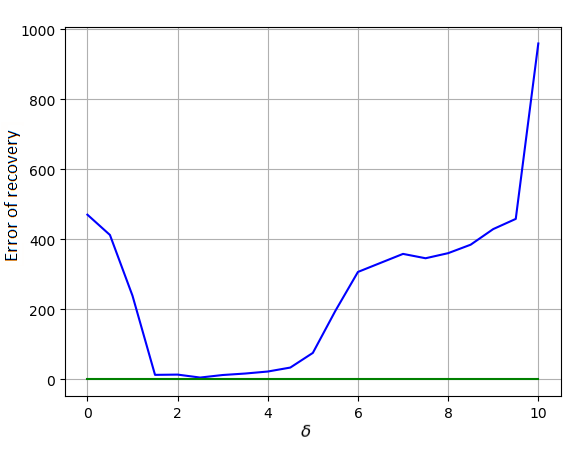
\includegraphics[width=0.9\textwidth]{./Pictures/ErrorRecoveryOK.PNG}
\caption{\small{Recovery of the true cluster structure using $3$ observations on a graph with generated with the stochastic block model with $3$ clusters and $50$ vertices. Each cluster has $8,17$ and $25$ vertices respectively. The probability to connect two edges inside a cluster is set to $p=0.65$ for all clusters. The probability to connect two edges not in the same cluster is $q=0.2$. Notice how perfect recovery (i.e recovery with error $0$) is achieved for some values of $\delta$. }}
 \label{fig:errorRecovery}
\end{figure}




Theorem \ref{thm: transport} assures that as long as $p_i > 0.5$ and $q< 0.5$ the probability of perfect recovery converges to $1$. The following experiments corroborate this result:
We fix $n=50$, $k=2$, and let the first cluster have $15$ vertices and the second one $35$. We let $p =  p_1 = p_2$ vary between $0.5$ and $1$ and $q$ vary between $0$ and $0.5$.  For each pair $(p,q)$, we generate $N$ observations, run our algorithm and measure the recovery error. We repeat this process $10$ times and store the mean error of recovery in a matrix.
We present the heat maps of such matrices in Figure~\ref{fig:Variapq} for different values of $N$. 


\begin{figure}[H]
\begin{tabular}{cc}
  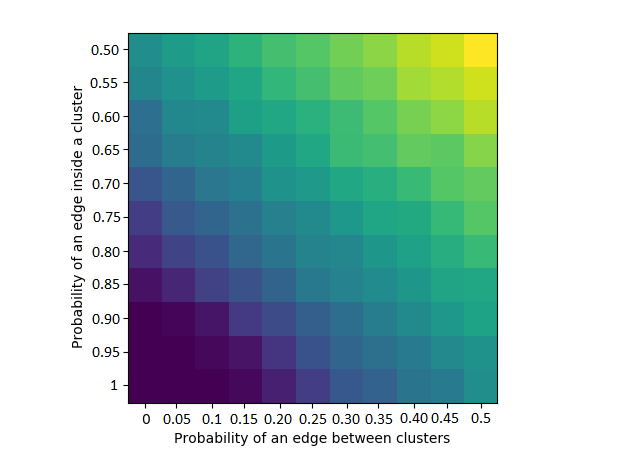
\includegraphics[width=85mm]{./Pictures/Variapq1.PNG} &   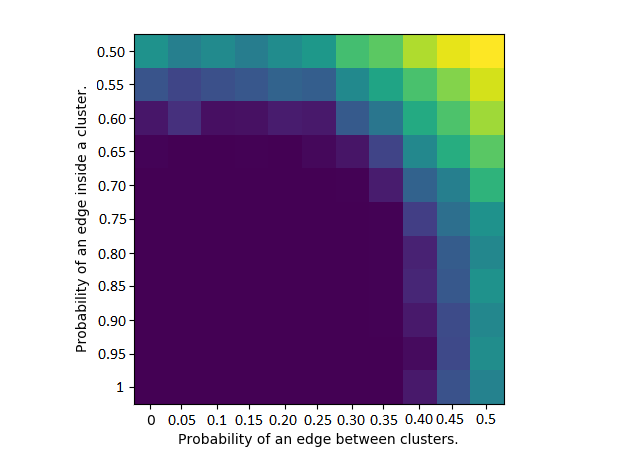
\includegraphics[width=85mm]{./Pictures/Variapq3.PNG} \\
(a) N=1 & (b) N=3 \\[6pt]
 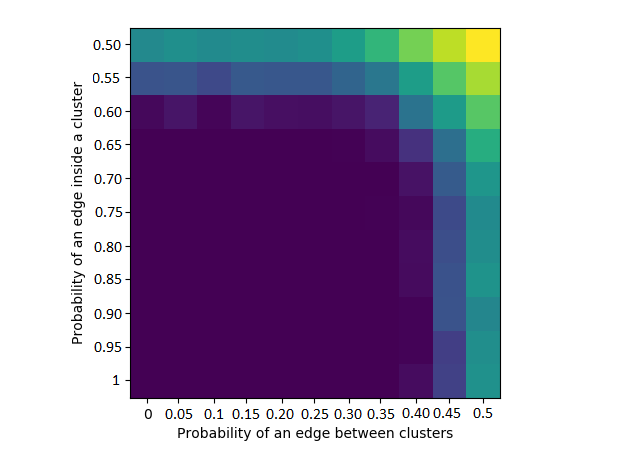
\includegraphics[width=85mm]{./Pictures/Variapq7.PNG} &   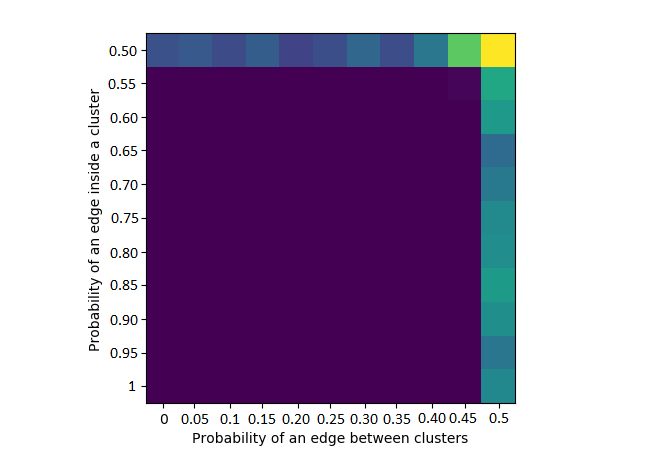
\includegraphics[width=85mm]{./Pictures/Variapq25.PNG} \\
(c) N=7 & (d) N=25\\[6pt]

\end{tabular}
\caption{Simulation results for the average error of recovery (over $10$ trials) for different values of $p$ and $q$ with $N$ observations. $\delta = 1.5$ for the first two figures and $0.8$ for the other two. Dark purple indicates 0 error while brighter colors indicate a higher error.}
        \label{fig:Variapq}
\end{figure}

In the proof of theorem \ref{thm: transport}, the use of the spectral norm was crucial. Still, one might ask if other norms (say the $1$-norm, $2$-norm or $\infty$-norm) can also recover the underlying cluster structure.

To check this, We fix $n=50$, $k=2$ where the first cluster has $15$ vertices and the second one has $35$. We let $p_1 = p_2 = 0.70$ and $q=0.2$. We compute the error of recovery for different values of $\delta$. For recovery using the nuclear norm, we use the algorithm given in the previous section. For the $1$-norm, $2$-norm and $\infty$-norm we use the \textit{Mosek}~\cite{Mosek} implementation on Julia. 
We also include the recovery error of the graph obtained by simply averaging the observations, which we call the mean graph.
We repeat this experiment twice. First with $3$ observations and then with $7$.
Results are shown in figure \ref{fig:differentNorms}.


\begin{figure}[H]
     \centering
     \begin{subfigure}[b]{1\textwidth}
         \centering
         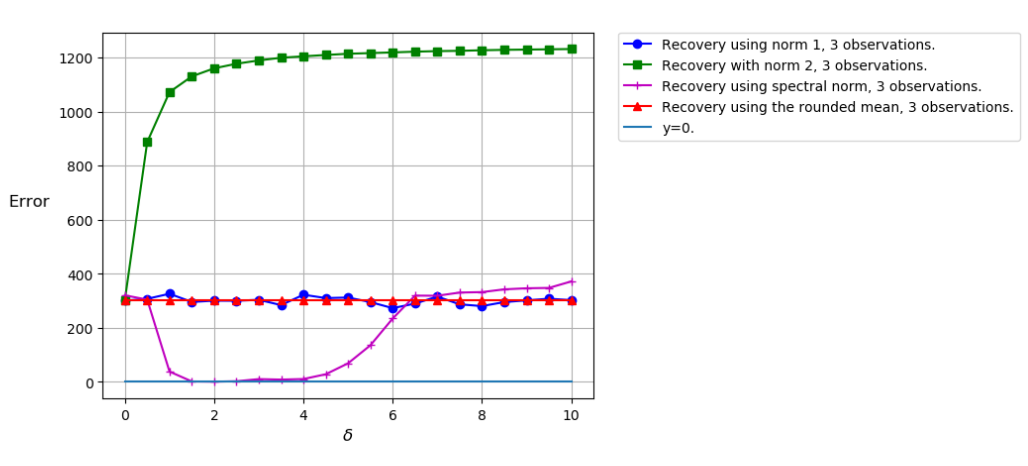
\includegraphics[width=\textwidth]{./Pictures/differentNorms.PNG}
\caption{$N=3$}
     \end{subfigure}
     \hfill
     \begin{subfigure}[b]{1\textwidth}
         \centering
         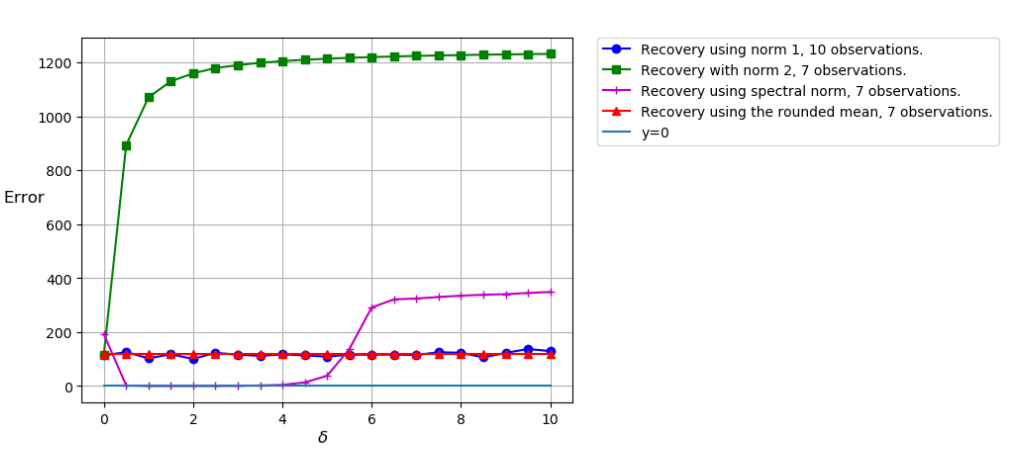
\includegraphics[width=\textwidth]{./Pictures/differentNorms7.PNG}
         \caption{$N=7$}
     \end{subfigure}
\caption{Error of recovery for different values of $\delta$ using the Wasserstein robust nuclear norm graph summarization and the $l_1$,$l_2$ norms as regularizers. The recovery error of the mean graph is also included.}
        \label{fig:differentNorms}
\end{figure}


Note that the recovery error of the mean graph decreases as more observations are considered. However it is still far off the true cluster structure even for 7 observations. By contrast, even with 3 observations our nuclear norm method is capable of recovering the true cluster structure in a wide range of $\delta$s. 
  
It is important to ask how fast does  the algorithm converge to the true cluster structure as the number of samples $N$ grows. The following figures show that this convergence occurs very quickly (at least for the stochastic block model), and thus that the Wasserstein summarization algorithm is a potentially useful approach.

\begin{figure}[H]
     \centering
     \begin{subfigure}[b]{0.8\textwidth}
         \centering
         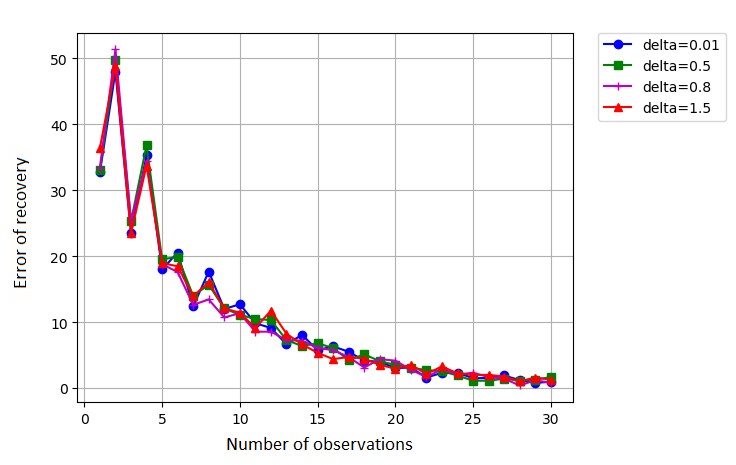
\includegraphics[width=\textwidth]{./Pictures/speedMean.PNG}
         \caption{Error of recovery using the mean graph.}
     \end{subfigure}
     \hfill
     \begin{subfigure}[b]{0.8\textwidth}
         \centering
         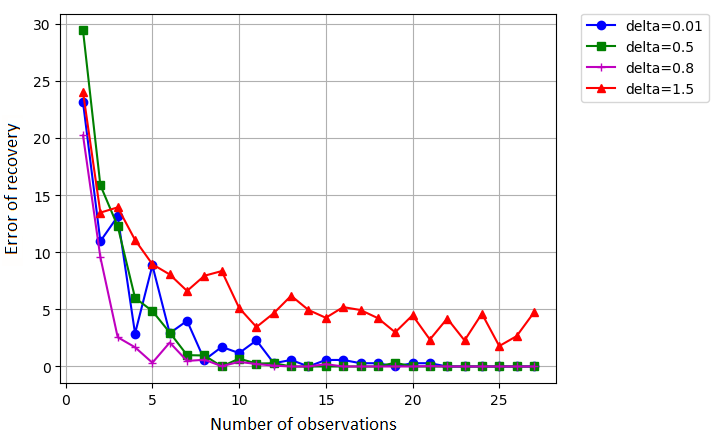
\includegraphics[width=\textwidth]{./Pictures/speedspectral.PNG}
         \caption{Error of recovery using the Wasserstein robust nuclear norm graph summarization.}
     \end{subfigure}
	\caption{Simulation results for the speed of convergence to the true cluster structure of the Wasserstein robust nuclear norm graph summarization versus the mean graph summarization .}
        \label{fig:speed}
\end{figure}


As $\delta$ varies, the recovered graph changes as well. Figure~\ref{fig:recupera} shows the recovered graphs for different values of $\delta$. Note that the optimum of our algorithm does not necessarily have entries in $\{0,1\}$ (except in the region with perfect recovery) and one might be tempted to round down the entries below certain threshold (say $0.4$) and round up those above another threshold (say $0.6$). However, it is not clear what to do with entries between both thresholds. 

\begin{figure}[H]
     \centering
     \begin{subfigure}[b]{0.35\textwidth}
         \centering
         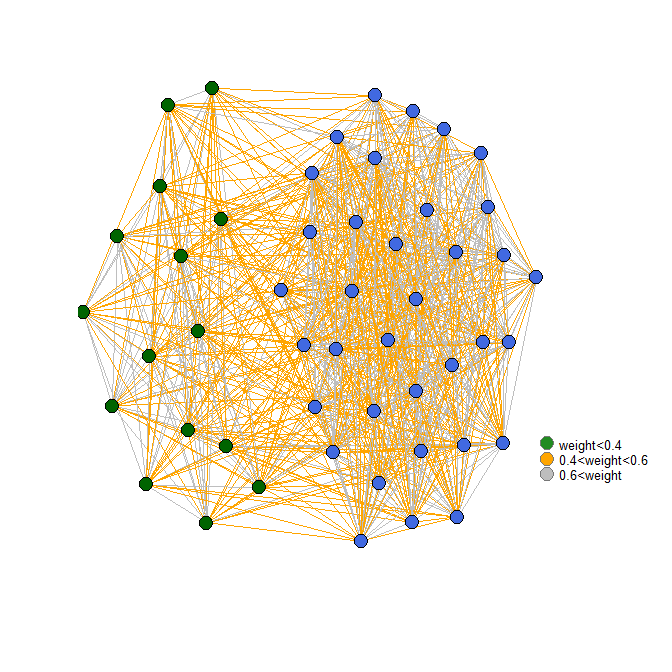
\includegraphics[width=\textwidth]{./Pictures/recupera0.png}
         \caption{Recovery with $\delta=0$}
     \end{subfigure}
     \hfill
     \begin{subfigure}[b]{0.37\textwidth}
         \centering
         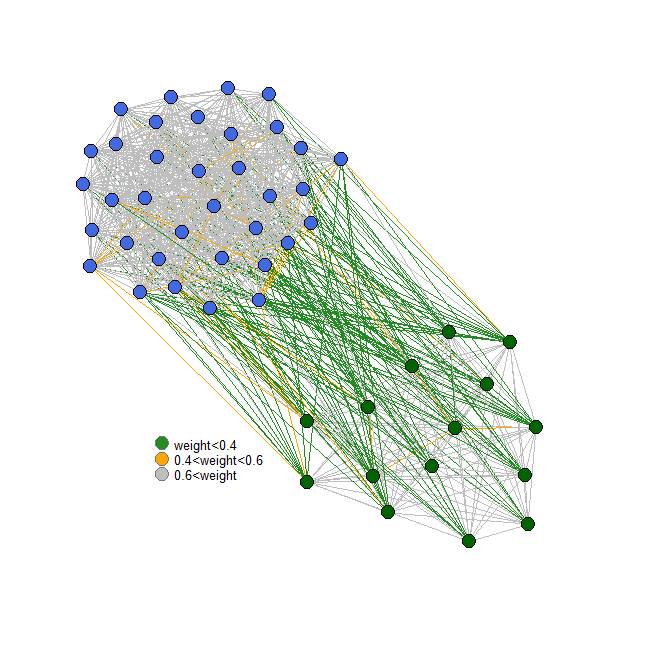
\includegraphics[width=\textwidth]{./Pictures/recupera1.png}
         \caption{Recovery with $\delta=0.1$}
     \end{subfigure}
     \hfill
     \begin{subfigure}[b]{0.37\textwidth}
         \centering
         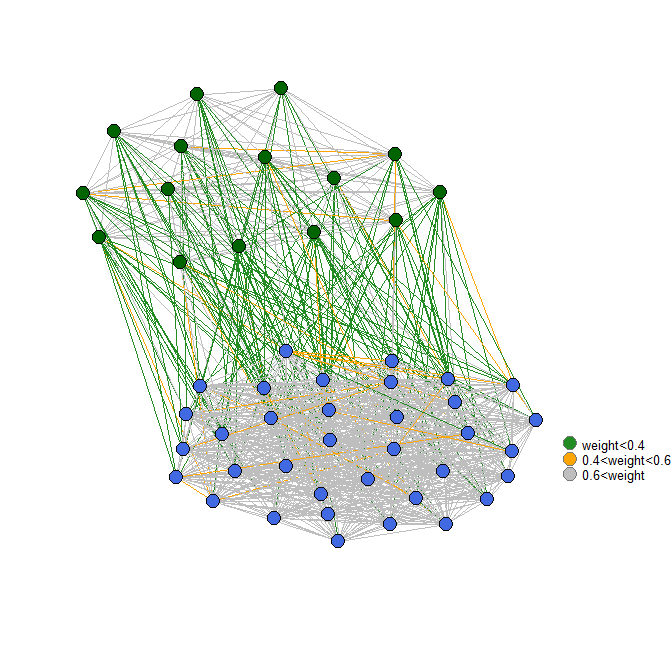
\includegraphics[width=\textwidth]{./Pictures/recupera2.png}
         \caption{Recovery with $\delta=0.5$}
     \end{subfigure}
     \hfill
     \begin{subfigure}[b]{0.37\textwidth}
         \centering
         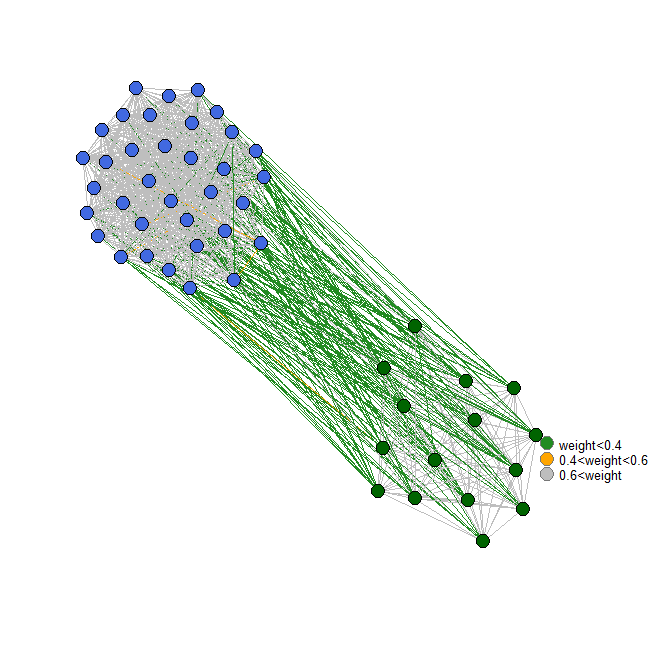
\includegraphics[width=\textwidth]{./Pictures/recupera4.png}
         \caption{Recovery with $\delta=1.2$}
     \end{subfigure}
     	\hfill
     \begin{subfigure}[b]{0.37\textwidth}
         \centering
         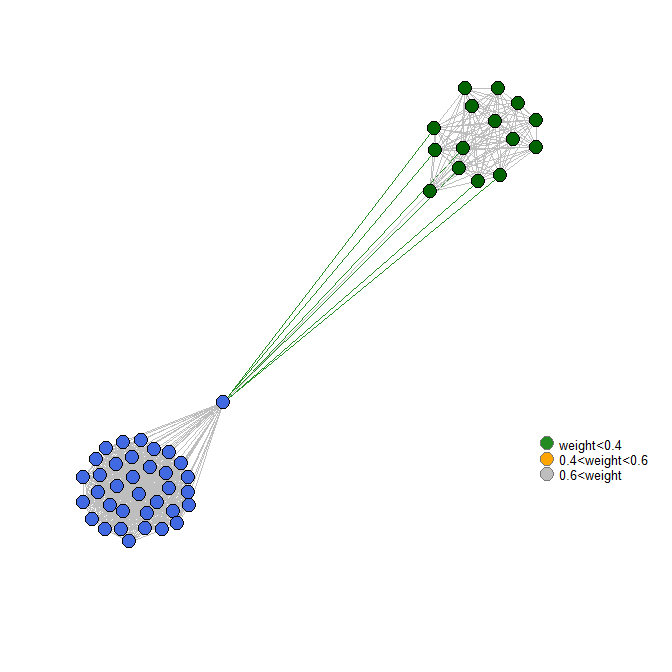
\includegraphics[width=\textwidth]{./Pictures/recupera5.png}
         \caption{Recovery with $\delta=1.5$}
     \end{subfigure}
     \hfill
     \begin{subfigure}[b]{0.37\textwidth}
         \centering
         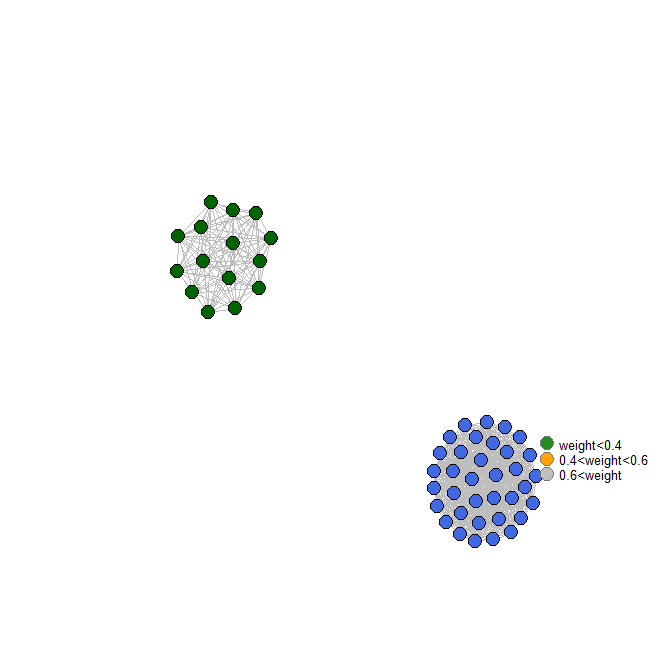
\includegraphics[width=\textwidth]{./Pictures/recupera6.png}
         \caption{Recovery with $\delta=2$}
     \end{subfigure}
     \hfill
     \begin{subfigure}[b]{0.37\textwidth}
         \centering
         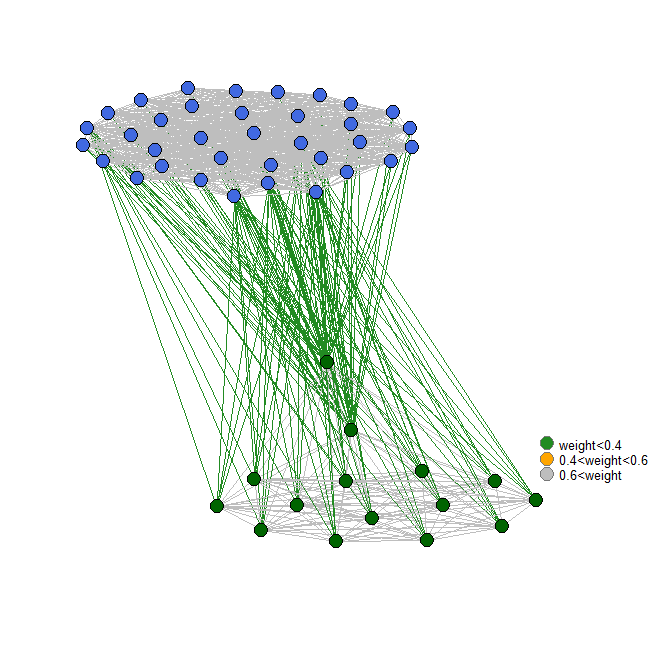
\includegraphics[width=\textwidth]{./Pictures/recupera7.png}
         \caption{Recovery with $\delta=11$}
     \end{subfigure}
      \hfill
     \begin{subfigure}[b]{0.37\textwidth}
         \centering
         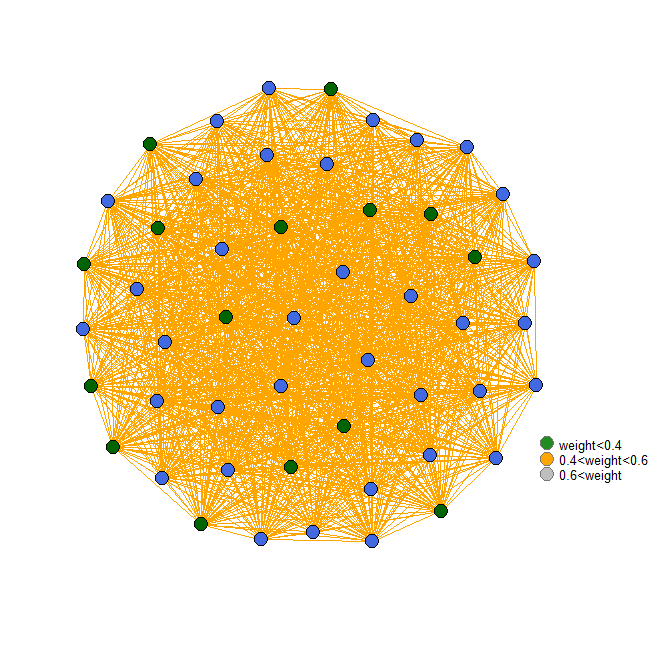
\includegraphics[width=\textwidth]{./Pictures/recupera8.png}
         \caption{Recovery with $\delta=14$}
     \end{subfigure}
        \caption{\small{Recovered graph from the same observations for different values of $\delta$. }}
        \label{fig:recupera}
\end{figure}








All Julia code used for building the simulations in this section is available at ~\url{https://github.com/Zlinki/WassersteinRobustSummarization}.















%\section{Some numerical examples using the stochastic block model.}
%\label{Numerics}
%\mv{Aca creo que deberia haber ejemplos de tres tipos:
%\begin{enumerate}
%\item De grafos chiquitos, digamos 20 vertices en los que se vea como cambia el \'optimo en la medida en que el par\'ametro $\delta$ va cambiando.
%\item En grafos medianos sus gr\'aficas comparativas de performance para diferentes m\'etricas con pocos samples
%\item En grafos grandes algo de cross-validation? Para ver como escoger el $\delta$? Me imagino que si uno va viendo que tan lejos esta de ser entera la solucion entonces uno puede encontrar un rango para $\delta$ donde da resultados ch\'everes.
%\end{enumerate}





\bibliographystyle{abbrv}
\bibliography{lit}

\end{document}


Our following Lemma gives us a decomposition Theorem for symmetric matrices. This decomposition will be very useful when computing spectral norms in the two-block case.
Suppose that we have only two blocks $C_1$ and $C_2$ and let $u$ be the vector given by
\[u_i=\begin{cases}
1\text{ if $i\in C_1$}
-1\text{ if $i\in C_2$}
\end{cases}
\]
Define $H^*:=uu^t$ and for $i=1,\dots, n$ let $e_{ii}$ be the $n\times n$ matrix whose only nonzero entry is in position $ii$ and has value $1$ 


\begin{lemma} Assume $|C_1|\neq |C_2|$ If $A$ is a symmetric matrix then there exist unique constants $\lambda_1,\dots, \lambda_{n-1}$ and a matrix $K$ such that $KH^*=H^*K=0$ such that
\[A= \frac{\langle H^*,A\rangle }{n^2} H^* +\sum_{i=1}^{n-1}\lambda_1(e_{i,i}-e_{i+1,i+1})+K.\]
And in particular the following equality holds  
\[ \|A\| =\max(A-K,K).\]
\end{lemma}
\begin{proof} The $n$ vectors in $v^tH^*$ and $v^t(e_{i,i}-e_{i+1,i+1})$ for $i=1,\dots, n-1$ are linearly independent in $\RR^n$ because the sum of the entries of all but the first one vanish. It follows that $v^tA$ can be expressed uniquely as a linear combination of them 


\end{proof}



\bibliographystyle{abbrv}
\bibliography{lit}



\end{document}


\section{Conclusions and future work}

In this paper, we presented the general problem of finding deterministic summaries from an independent sample of a random graph $\mathcal{G}$. We then specialized this problem to the case of community detection and showed how the Wasserstein metric allows us to reformulate this problem as a robust optimization problem. We showed that if the Wasserstein distance is induced by the nuclear norm, we can recover the exact cluster structure of random graphs generated with the stochastic block model with overwhelming probability with very few samples. We presented a specific algorithm to solve the \textit{Wasserstein robust nuclear norm summarization problem} and gave substantial simulations that corroborate our theoretical results.

Most importantly, we showed that a well studied problem in machine learning can be recast as a robust optimization problem using the Wasserstein metric. This approach is very promising, as it gives a principled approach to machine learning \mv{quite la puya a deep learning. Nunca digas de esta agua no beber\'e}. For example, see \cite{ColumbiaAlvaro}. This work is a small contribution to the growing body of applications of optimal transport to machine learning.



We conclude by briefly mentioning three interesting problems that rose in development of  this work. 
\textbf{Sparse regime in community detection.} In the literature, the problem of finding communities in the stochastic block model when the graph is sparse is well studied. For example, see \cite{krzakala2013spectral}. How does sparsity affect our results? We suspect that our algorithm are not well suited for sparse matrix since our methods are based on splitting the observations in sparse plus low rank matrices, and thus identifiability problems would rise if the observed matrices were sparse to begin with. 

\textbf{Arbitrary distribution of the} $\Gamma_{ij}$. The quantities $\Gamma_{ij}$ presented in \ref{Sec: subdifferential} are random variables whose distribution is given by the properties of the stochastic block model. It would be interesting to study random graphs where the $\Gamma_{ij}$ have an arbitrary distribution. This could lead to an application of our methods to weighted graphs, or to an appealing class of random graphs. 


\textbf{Graph summarization in an adversarial setting.} It would be interesting to explore graph summarization on a broader setting. For example, we could consider an adversarial setting, where  and adversary is presented a graph with a certain structure(for example a tree structure) and he generates a sample of graphs by removing or adding edges on the graph with probability $q< 1/2$. Can we recover the original graph given a very small sample? If so, which representable convex function would allow us to properly recover the structure (as is the case of the nuclear norm and the community structure) ? Is it enough that such a function has a rich subdifferential as the nuclear norm so that some version of theorem \ref{thm: transport} applies?





%\mv{Como extendemos este razonamiento al caso de tres o m\'as clusters? Debe ser posible utilizar otras matrices de transporte para este caso que vivan en el kernel. Algo interesante es que con tres clusters es necesario que los promedios de una matriz aniquilada por $H^*$ dentro de cada uno de los bloques $C_i\times C_j$ deban ser cero.} 

Next we will now prove the case when there are any number of clusters. The proof will be similar that of the previous theorem. We will start with the candidate matrix $\frac{-2\delta}{n}H^*$ and correct it by adding transportation matrices that assure that the corrected matrix belongs to the subdifferential of $\Delta(A)$ at $A^*$.
The difficulty in applying the tools of the previous theorem to solve the general case is that the matrices $K$ that transport weight from one cluster to another do not, in general, satisfy the relation $KH^* = H^*K = 0$ when there are more than two clusters. This problem can be solved by splitting the matrix $H^*$ into matrices than only take into account $2$ clusters, and using the previous theorem.
We begin recalling the following simple result:

\begin{lemma}
Let $a_i,b_i \geq 0, \ i = 1,\dots,p$ be two non-negative, finite sequences of real numbers such that
\[
\sum_{i=1}^{p}a_i \geq \sum_{i=1}^{p}b_i.
\]
Then there exist a finite sequence of reals $c_i$ such that
\begin{itemize}
\item $\sum_{i=1}^p c_i=0.$
\item $a_i \geq b_i+c_i \  \forall i.$
\end{itemize}
\end{lemma}


Now we proceed to do the proof. For  clusters $C_s\neq C_t$ define the matrix $H^{C_sC_t}$ whose entries are given by: 
\[
H^{C_iC_j}_{uv}= 
\begin{cases}
1 \text{ if } u,v \in C_s \text{ or } u,v \in C_t. \\
-1 \text{ if } u \in C_s, v \in C_t \text{ or } u \in C_s, v\in C_t. \\
0 \text{ in any other case.}
\end{cases}
\]
Notice that this matrix has $4$ blocks. Two with only $1$ and two with only $-1$. Moreover, its spectral norm is equal to $|C_s+|C_t|$.

\begin{theorem}\label{lemma: transport2}
Suppose that $ b(\Gamma,\delta) < min(\delta,a(\Gamma,\delta))$.Then,
$A^*$ is a minimizer of the optimization problem $\min_A\Delta(A)$. 
\end{theorem}

\begin{proof}

Assume that there are $l$ clusters. First of all, observe that
\[
\frac{-2\delta}{n}H^* = \frac{-2\delta}{n}\frac{1}{l-1}\sum_{1\leq s<t\leq l}H^{C_sC_t}.
\]
For each, $C_s\neq C_t$ construct a transport matrix $\Delta_{st}$ as in the previous theorem, as to assure that $\Delta_{st}H^{C_sC_t} = H^{C_sC_t} \Delta_{st}=0$. This can be done since $H^{C_sC_t}$ takes into account only two clusters. Recall that the total amount of weight to be corrected is $b(\Gamma,\delta)$. Let $w_{s,t}$ the weight to be distributed from cluster $s$ to cluster $t$. In the notation of the previous theorem, $w_{st}$ is just the sum of the 
$\gamma_{l_p}^{ij}$ where $l_p\in C_s $ and $ij \in C_t $.


Let 

\[
C:= -\frac{2\delta}{n}H^* + \sum_{i<j}\Delta_{ij} = \frac{-2\delta}{n}\frac{1}{l-1}\sum_{1\leq i<j\leq l}H^{C_iC_j} + \sum_{i<j}\Delta_{ij}
\]

Finally, assume that for each $i<j$, $\frac{1}{l-1}||H^{C_iC_j}||\geq ||\Delta_{ij}||$.

Then,
\[
\begin{aligned}
\left\|C\right \| & = \left\| \frac{-2\delta}{n}\frac{1}{l-1}\sum_{1\leq i<j\leq l}H^{C_iC_j} + \sum_{i<j}\Delta_{ij}  \right \|  \\ & \leq \frac{2\delta}{n(l-1)}\sum_{1\leq i<j\leq l}\left \|H^{C_iC_j}+ \frac{n(l-1)}{2\delta} \Delta_{ij}\right \|  \\
& = \frac{2\delta}{n(l-1)}\sum_{1\leq i<j\leq l} \max (\left\|H^{C_iC_j}\right\|,\left\|\frac{n(l-1)}{2\delta}\Delta_{ij}\right\|)& \\
\end{aligned}
\]
Now notice that 
\[
\begin{aligned}
\delta \geq b(\Gamma,\delta) \text{ therefore } (l-1)n & \geq \frac{(l-1)n}{\delta} b(\Gamma,\delta) \\\text{ which implies that }  \sum_{i<j}\left \|H^{C_iC_j}\right \|  & \geq  \frac{(l-1)n}{\delta}\sum_{i<j}w_{i,j}   \\
 & \geq \frac{(l-1)n}{2\delta}\sum_{i<j}\left \|\Delta_{i,j} \right \|  .
\end{aligned}
\]
By the claim, we can assume without loss of generality that
for each $i<j$,
\[
\left \|H^{C_i,C_j}\right \| \geq  \frac{(l-1)n}{\delta}\left \|\Delta_{i,j} \right \|.
\]

This implies that the last sum reduces to
\[
\frac{2\delta}{n(l-1)}\sum_{1\leq i<j\leq l} \left\|H^{C_iC_j}\right\| = \sum_{1\leq i<j\leq l} \frac{2\delta(|C_i|+|C_j|)}{n(l-1)} = \frac{2\delta(l-1)}{n(l-1)}\sum_{1\leq i<j\leq l}|C_i|+|C_j|=2\delta.
\]
And so
$\|C\| \leq 2\delta$.

\end{proof}
\ddr{toca revisar que $<h^*,C>$ es igual a $-2\delta n$ o eso es obvio?}
\mv{Toca revisar. Porfa revisa y me cuenta}
\begin{remark}
In practice, $\delta$ could be chosen by using a trial and error methodology, along with a cluster quality metric. One such metric is called the \textit{silhouette}.
\end{remark}



\begin{figure}
     \centering
     \begin{subfigure}[b]{0.5\textwidth}
         \centering
         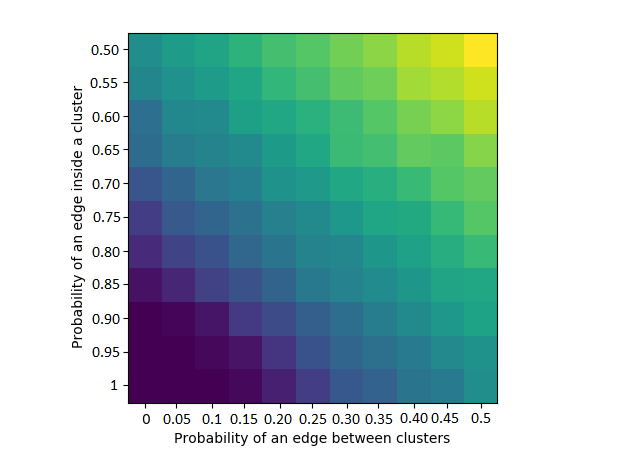
\includegraphics[width=\textwidth]{./Pictures/Variapq1.PNG}
         \caption{$N=1$}
     \end{subfigure}
     \hfill
     \begin{subfigure}[b]{0.5\textwidth}
         \centering
         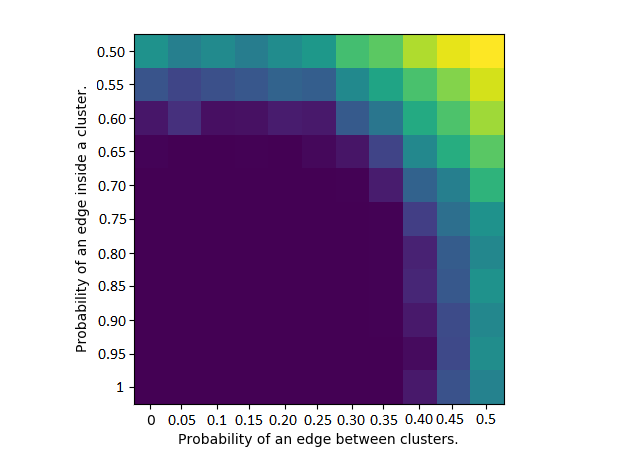
\includegraphics[width=\textwidth]{./Pictures/Variapq3.PNG}
         \caption{$N=3$}
     \end{subfigure}
     \hfill
     \begin{subfigure}[b]{0.5\textwidth}
         \centering
         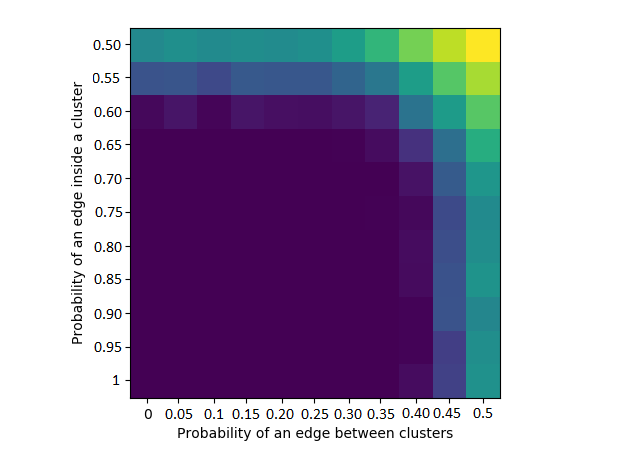
\includegraphics[width=\textwidth]{./Pictures/Variapq7.PNG}
         \caption{$N = 7$}
     \end{subfigure}
     \hfill
     \begin{subfigure}[b]{0.5\textwidth}
         \centering
         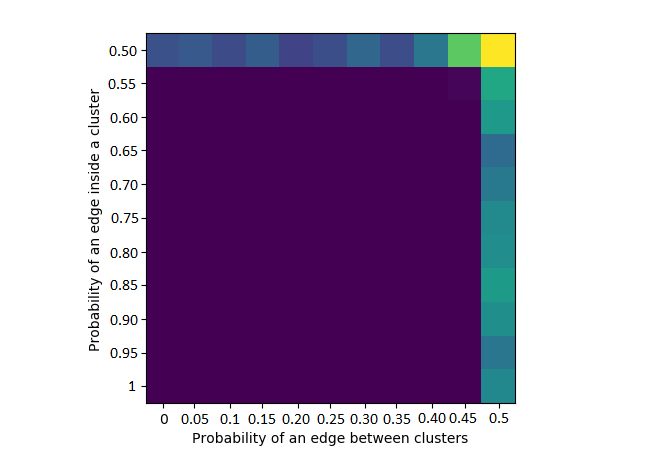
\includegraphics[width=\textwidth]{./Pictures/Variapq25.PNG}
         \caption{$N = 25$}
     \end{subfigure}
        \caption{Simulation results for the average error of recovery (over $10$ trials) for different values of $p$ and $q$ with $N$ observations. $\delta = 1.5$ for the first two figures and $0.8$ for the other two. Dark purple indicates 0 error while brighter colors indicate a higher error.}
        \label{fig:Variapq}
\end{figure}


